\documentclass[12pt,a4paper]{report}
\usepackage[english]{babel}
\usepackage{newlfont}
\usepackage{color}
\usepackage{graphicx} % figures...
\usepackage{amsmath} % math symb
\newcommand{\norm}[1]{\left\lVert#1\right\rVert} % norm sign
\usepackage{enumerate}
\usepackage{url}
\usepackage{lipsum} % fake text
\usepackage{gensymb} % ° symbol
\usepackage{bm} % bold math symbols
\usepackage{amssymb} % calligraphy
\usepackage{color,soul} % highlighting text
\usepackage[labelfont={bf,it},textfont=it, margin=1cm]{caption} % caption settings
\usepackage{subcaption} % subfigures
\usepackage{natbib} % biblio
\bibliographystyle{plain}
\usepackage[nottoc]{tocbibind} % show bib in toc
\usepackage{hyperref} % show intro in toc

\textwidth=450pt
\oddsidemargin=0pt

\begin{document}
\begin{titlepage}
\begin{center}
{{\Large{\textsc{Alma Mater Studiorum $\cdot$ University of  Bologna}}}}
\rule[0.1cm]{15.8cm}{0.1mm}
\rule[0.5cm]{15.8cm}{0.6mm}
\\\vspace{3mm}
{\small{\bf School of Science \\
Department of Physics and Astronomy\\
Master Degree in Physics}}
\end{center}

\vspace{23mm}

\begin{center}
    \LARGE{\bf Dataset Generation for the Training of Neural Networks Oriented toward Histological Image Segmentation}\\
\end{center}

\vspace{40mm} \par \noindent

\begin{minipage}[t]{0.47\textwidth}
    {\large{\bf Supervisor: \vspace{2mm}\\
    Dr. Enrico Giampieri\\\\
    \bf Co-supervisor: \vspace{2mm}\\
    Dr. Nico Curti\\\\}}
\end{minipage}

%
\hfill
%
\begin{minipage}[t]{0.47\textwidth}\raggedleft
    \textcolor{black}{
        {\large{\bf Submitted by:
            \vspace{2mm}\\
            {Alessandro d'Agostino}}}
    }
\end{minipage}

\vspace{21mm}

\begin{center}
Academic Year 2019/2020
\end{center}
\end{titlepage}

% \null\vspace{\stretch{1}}
    \begin{flushright}
    Acknowledgements:
    \end{flushright}
\vspace{\stretch{2}}\null

\chapter*{Abstract}
The project is inspired by an actual problem of timing and accessibility in the analysis of histological samples in the health-care system. In this project, I address the problem of synthetic histological image generation for the purpose of training Neural Networks for the segmentation of real histological images. The collection of real histological human-labeled samples is a very time consuming and expensive process and often is not representative of healthy samples, for the intrinsic nature of the medical analysis. The method I propose is based on the replication of the traditional specimen preparation technique in a virtual environment. The first step is the creation of a 3D virtual model of a region of the target human tissue. The model should represent all the key features of the tissue, and the richer it is the better will be the yielded result. The second step is to perform a sampling of the model through a virtual tomography process, which produces a first completely labeled image of the section. This image is then processed with different tools to achieve a histological-like aspect. The most significant aesthetical post-processing is given by the action of a style transfer neural network that transfers the typical histological visual texture on the synthetic image. This procedure is presented in detail for two specific models: one of pancreatic tissue and one of dermal tissue. The two resulting images compose a pair of images suitable for a supervised learning technique. The generation process is completely automatized and does not require the intervention of any human operator, hence it can be used to produce arbitrary large datasets. The synthetic images are inevitably less complex than the real samples and they offer an easier segmentation task to solve for the NN. However, the synthetic images are very abundant, and the training of a NN can take advantage of this feature, following the so-called curriculum learning strategy.


\tableofcontents{}

\chapter*{Introduction}
In the last decades, the development of Machine Learning (ML) and Deep Learning (DL) techniques has contaminated every aspect of the scientific world, with interesting results in many different research fields. The biomedical field is no exception to this and a lot of promising applications are taking form, especially as Computer-Aided Detection (CAD) systems which are tools for the support of physicians during the diagnostic process. Medical doctors and the healthcare system in general collect a huge amount of data from patients during all the treatment, screening, and analysis activities in many different shapes, from anagraphical data to blood analysis to clinical images.

In medicine, the study of images is ubiquitous and countless diagnostic procedures rely on it, such as X-ray imaging (CAT), nuclear imaging (SPECT, PET), Magnetic resonance, and visual inspection of histological specimens after biopsies. The branch of artificial intelligence in the biomedical field that handles image analysis to assist physicians in their clinical decisions goes under the name of Digital Pathology Image Analysis (DPIA).
In this thesis work, I want to focus on some of the beneficial aspects introduced by DPIA in the histological images analysis and some particular issues in the development of DL models able to handle this kind of procedure.

Nowadays the great majority of analysis of histological specimens occurs through visual inspection, carried out by highly qualified experts. Some analysis, as cancer detection, requires the ability to distinguish if a region of tissue is healthy or not with high precision in very wide specimens. This kind of procedure is typically very complex and requires prolonged times of analysis besides substantial economic efforts. Furthermore, the designated personnel for this type of analysis is often limited, leading to delicate issues of priority assignment while scheduling analysis, based on the estimated patient's clinical development. Some sort of support to this analysis procedure is therefore necessary.

The problem of recognizing regions with different features within an image and detect their borders is known in computer vision as the segmentation task, and it's quite widespread with countless different applications, allowing a sort of automatic image interpretation. In ML the segmentation problem is usually faced as a supervised task, hence the algorithm in order to be trained properly requires an appropriate quantity of pre-labeled images, from which learn the rules through which distinguish different regions. This means that the development of segmentation algorithms for a specific application, as would be the one on histological images, would require a lot of starting material, previously analyzed from the same qualified expert encharged of the visual inspection mentioned before. A human operator thus is required to manually track the boundaries, for example, between healthy and tumoral regions within a sample of tissue and to label them with their identity, as in Figure \ref{fig:man_seg}. The more the algorithm to train is complex the more starting material is required to adjust the model's parameters and reach the desired efficacy.

\begin{figure}
    \centering
    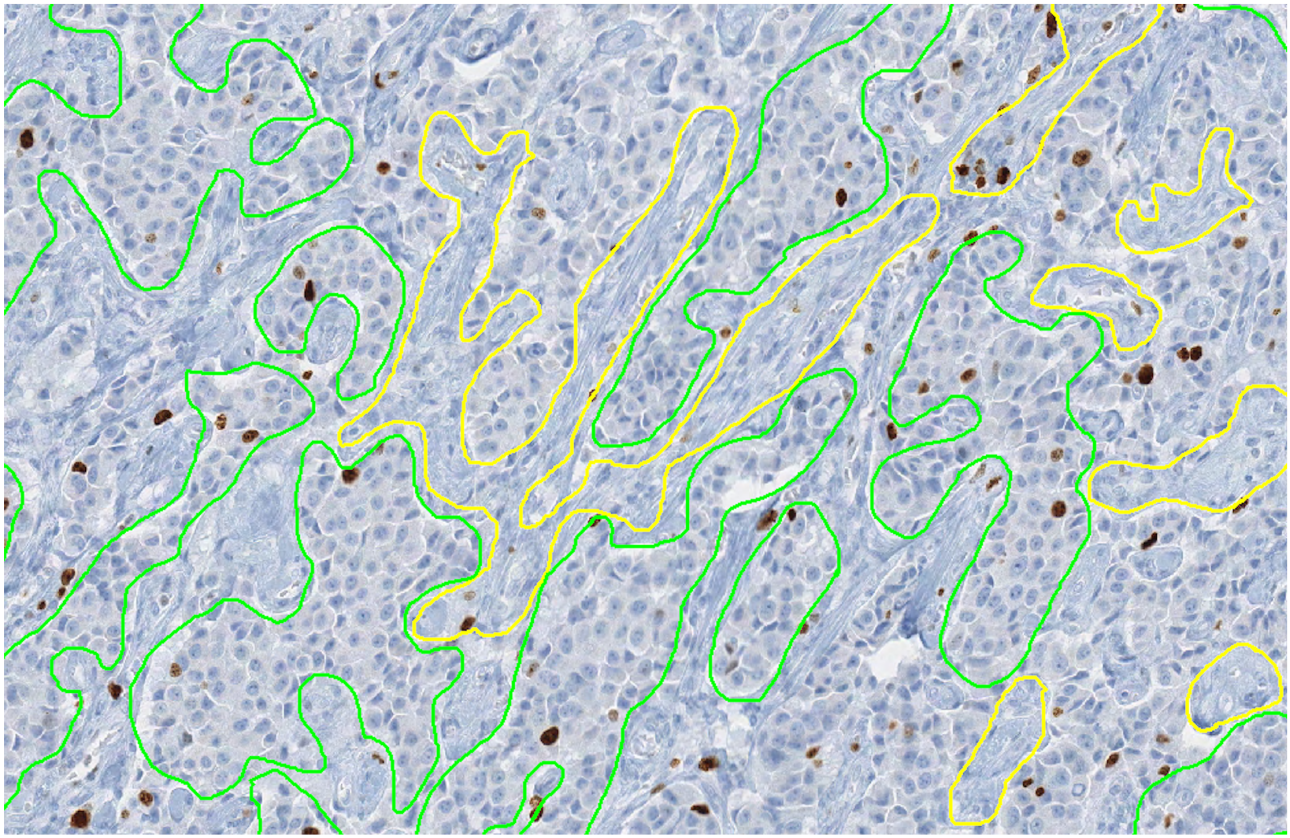
\includegraphics[width = 0.9\textwidth]{images/manual_seg}
    \caption{Interleaving of tumor (green annotation) and non-tumor (yellow annotation) regions \cite{Ki67}.}
    \label{fig:man_seg}
\end{figure}


The latest developed segmentation algorithms are based on DL techniques, hence based on the implementation of intricated Neural Networks (NN) which process the input images and produce the corresponding segmentation. Those models are typically very complex, with millions of parameters to adjust and tune, therefore they need a huge amount of pre-labeled images to learn their segmentation rules. This need for data is exactly the main focus of my thesis work. The shortage of ground truth images is indeed one of the toughest hurdles to overcome during the development of DL-based algorithms. Another important aspect to bear in mind is the quality of the ground truth material. It's impossible for humans to label boundaries of different regions with pixel-perfect precision, while for machines the more precise is the input the more effective is the resulting algorithm.


Different approaches have already been explored to overcome this problem, and they are mainly based on the generation of synthetic labeled data to use during the training phase. Some techniques achieve data augmentation manipulating already available images and then generating \textit{new} images, but as we will see later this approach suffers from different issues. The technique that I propose in this work follows a generation from scratch of entire datasets suitable for the training of new algorithms, based on the 3D modelization of a region of human tissue at the cellular level. The entire traditional sectioning process, which is made on real histological samples, is recreated virtually on this virtual model. This yields pairs of synthetic images with their corresponding ground-truth. Using this technique one would be able to collect sufficient material for the training (the entire phase or the preliminary part) of a model, overcoming the shortage of hand-labeled data.

The 3D modeling of a region of particular human tissue is a very complex task, and it is almost impossible to capture all the physiological richness of a histological system. The models I implemented thus are inevitably less sophisticated respect the target biological structures. I'll show two models: one of pancreatic tissue and another of dermal tissue, besides all the tools I used and the choices I made during the designing phase.

In order to present organically all the steps of my work the thesis is organized in chapters as follows:

\begin{enumerate}
    \item Structure

    \item Of the

    \item Thesis
\end{enumerate}


% \begin{enumerate}
%     \item Description of how histological images are obtained and analyzed, and which are the important aspects to take care of.
%     \item Thorough description of my model for the generation of synthetic images of pancreatic tissue
%     \item Thorough description of my model for the generation of synthetic images of epidermic tissue
%     \item Introduction to Deep Learning and Segmentation task, and state of the art of DL based segmentation algorithms.
%     \item Future work and improvements
% \end{enumerate}

\clearpage

\clearpage

\chapter{Histological Images Analysis}
    \hl{PREAMBLE TO THE FIRST CHAPTER. DESCRIPTION OF SECTIONS 1.1.x}

In sections 

    \section{Histological Images} \label{ssec:hist_im}

Modern histopathology is essentially based on the careful interpretation of microscopic images, with the intention of correctly diagnose patients and to guide therapeutic decisions. In the last years, thanks to the quick development of scanning techniques and image processing, the discipline of histology have seen radical improvements: the main of which undoubtedly is the passage from the microscope's oculars to the computer's screen. This digitalization process has brought several advantages, that were previously impossible in classical histology, like telepathology and remote assistance in diagnosis processes, the integration with other digitalized clinical workflows, and patients' history, but mainly the opening to applications of artificial intelligence.
The name Whole Slide Imaging (WSI) refers to the modern virtual microscopy discipline, which consists of scanning a complete microscope slide and creating a single high-resolution digital file. This is commonly achieved by capturing many small high-resolution image tiles or strips and then montaging them to create a full image of a histological section. The four key steps of this process are image acquisition (scansion), activation, editing, and on-screen image visualization.

In the field of Digital Pathology (DP) an essential concept in image understanding is the magnification factor, which indicates the scale of representation of the image and allows dimension referencing. This factor is usually indicated as the magnification power of the microscope's lenses used during the analysis. After the digitalization process, this original magnification factor is prone to change, depending on the resolution of the visualization screen. Therefore, image resolution is measured in $\mu m$ per pixel, and it is set by the different composition of the acquisition chain, as the optical sensor and the lenses. Histological scanner are usually equipped with 20$\times$ or 40$\times$ objectives, which correspond to 0.5 and 0.25 $mm$/pixels resolution values. Lenses with 20$\times$ magnification factor are the most suitable for the great majority of histopathological evaluations, and it is the golden standard for scansions, for its good trade-off between image quality and time of acquisition. Scansions with 40$\times$ magnification could increase four-fold acquisition and processing time, final file's dimension, and storage cost. A single WSI image, acquired with 20$\times$ will occupy more than 600 MB alone.

\begin{figure}
    \centering
    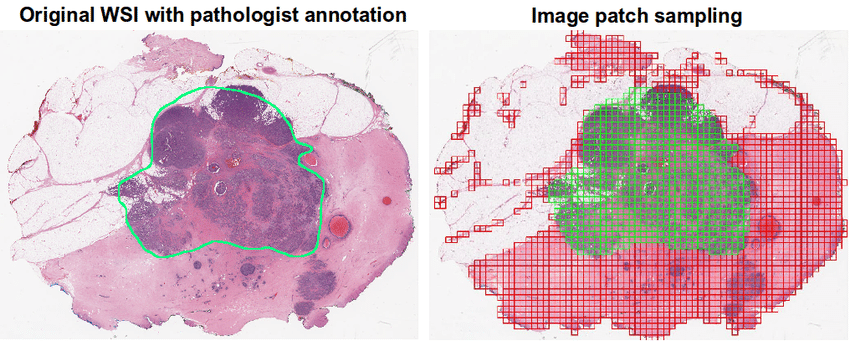
\includegraphics[width = \textwidth]{images/patches_grid}
    \caption{An example of whole slide image, with its grid decomposition in patches. It is visible the correspondence between a region of intereste maually anotated and the patches that matches that region. From \cite{WSI_grid}}
    \label{fig:patches_grid}
\end{figure}

Despite the WSI is a relatively mature discipline, it still struggles to integrate itself in the standard primitive diagnosis phase in histopathological laboratories. This is due primarily due to some disadvantages, like images'resolution, image compression's artifacts, and auto-focusing algorithms, which plays a key role in the specimen interpretation. Furthermore, the scansion of histological samples is an additional step in the analysis which takes time. Despite the technological improvements the average time for the acquisition of a sample is around 5/10 minutes, depending on the number of slices in the slide, for just a single level of magnification. While in traditional histology, the pathologist has access to all the magnification levels at the same time, in regions where it matters. The real advantage, in fact, is in the long term. Once the images have been acquired they can be archived and consulted remotely almost instantaneously, helping clinical analysis and allowing remote assistance, (telemedicine). Furthermore, the images now can be processed by artificial intelligence algorithms, allowing the application of technologies like Deep Learning which could revolutionize the research field, as already has been on many different disciplines in the scientific world.

In order to allow to automatically process, such big images as the ones obtained through WSI, it is necessary to subdivide them in smaller patches. The dimension of which should be big enough to allow interpretation and to preserve a certain degree of representability of the original image. In Figure \ref{fig:patches_grid} is shown an example of whole slide image, with its grid decomposition in patches. If the patches are too small, it should be over-specified for a particular region of tissue, loosing its general features. This could lead the learning algorithm to misinterpretation. However, this is not an exclusive limit of DP, for a human pathologist would be impossible too to make solid decisions on a too limited sample of tissue. After the subdivision in patches, a typical process for biomedical images is the so-called \textit{data augmentation} of images, that is the process of creating re-newed images from the starting material through simple geometrical transformations, like translation, rotation, reflection, zoom in/out. This technique is often implemented to avoid the \textit{overfitting}, which is the condition in which the model over-specialized its knowledge and lose the ability to generalize on new, unseen material, which reduces the effectiveness of the model. In section \ref{ssec:soa_seg} some actual model for biomedical image processing will be shown in detail.

 \begin{figure}
     \centering
     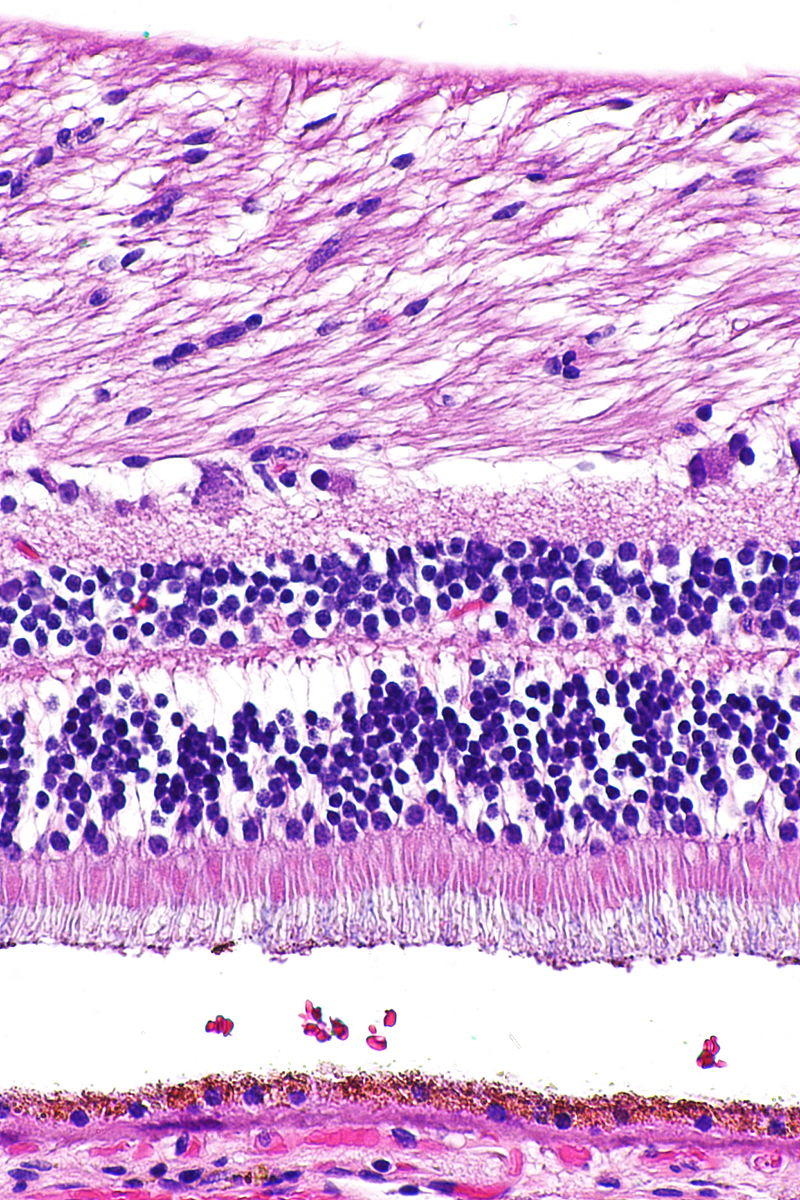
\includegraphics[width = 0.3\textwidth]{images/h&e_retyna}
     \caption{A sample of tissue from a retina (a part of the eye) stained with hematoxylin and eosin, cell nuclei stained blue-purple and extracellular material stained pink.}
     \label{fig:he_retyna}
 \end{figure}

\subsection{Slides Preparation for Optic Microscopic Observation} \label{ssec:samp_prep}
In modern, as in traditional histology, regardless on the fianl support of the image the sample has to be physically prepared, starting from the sample of tissue. The sample and slide preparation is a crucial step for histological or cytological observation. It is essential to highlight what needs to be observed and to \textit{immobilize} the sample at a particular point in time and with characteristics close to those of its living state. There are five key steps for the preparation of samples \cite{Alturkistani2015}:
\begin{description}
    \item [1) Fixation] is carried out immediately after the removal of the sample to be observed. It is used to immobilize and preserve the sample permanently in as life-like a state as possible. It can be performed immersing the biological material in a formalin solution or by freezing, so immersing the sample in a tissue freezing medium which is then cooled in liquid nitrogen.

    \item [2) Embedding] if the sample has been stabilazed in a fixative solution, this is the subsequent step. It consists in hardening the sample in a paraffin embedding medium, in order to be able to carry out the sectioning. It is necessary to dehydrate the sample beforehand, by replacing the water molecules in the sample with ethanol.

    \item [3) Sectioning] Sectioning is performed using microtomy or cryotomy. Sectioning is an important step for the preparation of slides as it ensures a proper observation of the sample by microscopy. Paraffin-embedded samples are cut by cross section, using a microtome, into thin slices of 5 $\mu m$. Frozen samples are cut using a cryostat. The frozen sections are then placed on a glass slide for storage at -80°C. The choice of these preparation conditions is crucial in order to minimize the artifacts. Paraffin embedding is favored for preserving tissues; freezing is more suitable for preserving DNA and RNA and for the labeling of water-soluble elements or of those sensitive to the fixation medium.

    \item [4) Staining] Staining increases contrasts in order to recognize and differentiate the different components of the biological material. The sample is first deparaffinized and rehydrated so that polar dyes can impregnate the tissues. The different dyes can thus interact with the components to be stained according to their affinities. Once staining is completed, the slide is rinsed and dehydrated for the mounting step.

\end{description}

Hematoxylin and eosin stain (H\&E) is one of the principal tissue stains used in histology \cite{he_stain}, and it is the most widely used stain in medical diagnosis and is often the gold standard \cite{Rosai2007}. H\&E is the combination of two histological stains: hematoxylin and eosin. The hematoxylin stains cell nuclei blue, and eosin stains the extracellular matrix and cytoplasm pink, with other structures taking on different shades, hues, and combinations of these colors. An example of H\&E stained is shown in Figure \ref{fig:he_retyna}, in which we can see the typical colour palette of an histological specimen.

    \clearpage
    \section{Introduction to Deep Learning}
Deep Learning is part of the broader framework of Machine Learning and Artificial Intelligence. Indeed all the problems typically faced using ML can also be addressed with DL techniques, for instance, regression, classification, clustering, and segmentation problems. We can think of DL as a universal methodology for iterative function approximation with a great level of complexity. In the last decades, this technology has seen a frenetic diffusion and an incredible development, thanks to the always increasing available computational power, and it has become a staple tool in all sorts of scientific applications.

\subsection{Perceptrons and Multilayer Feedforward Architecture}
Like other artificial learning techniques, DL models aim to \textit{learn} a relationship between some sort of input and a specific kind of output. In other words,  approximating numerically the function that processes the input data and produces the desired response. For example, one could be interested in clustering data in a multidimensional features space, or the detection of objects in a picture, or text manipulation/generation. The function is approximated employing a greatly complex network of simple linear and non-linear mathematical operations arranged in a so-called Neural Network (typically with millions of parameters). The seed idea behind this discipline is to recreate the functioning of actual neurons in the human brain: their entangled connection system and their "ON/OFF" behavior \cite{10.5555/3275328}.

The fondamental unit of a neural network is called perceptron, and it acts as a digital counterpart of a human neuron. As shown in Figure \ref{fig:perceptron} a perceptron collects in input a series on $n$ numerical signals $\vec{x} = 1, x_1, ..., x_n $ and computes a linear wieghted combination with the weights vectors $\vec{w} = w_0, w_1, ..., w_n$, where $w_0$ is a bias factor:

\begin{equation}
    f(\vec{x},\vec{w}) = \chi(\vec{x} \cdot \vec{w}).
\end{equation}

The results of this linear combination are given as input to a non-linear function $\chi(x)$ called the activation function. Typical choices as activation function are any sigmoidal function like $sign(x)$ and $tanh(x)$, but in more advanced applications other functions like ReLU \cite{1803.08375} are used. The resulting function $f(\vec{x},\vec{w})$ has then a simple non linear behaviour. It produces a binary output: 1 if the weighted combination is high enough and 0 if it is low enough, with a smooth modulation in-between the two values.

\begin{figure}
    \centering
    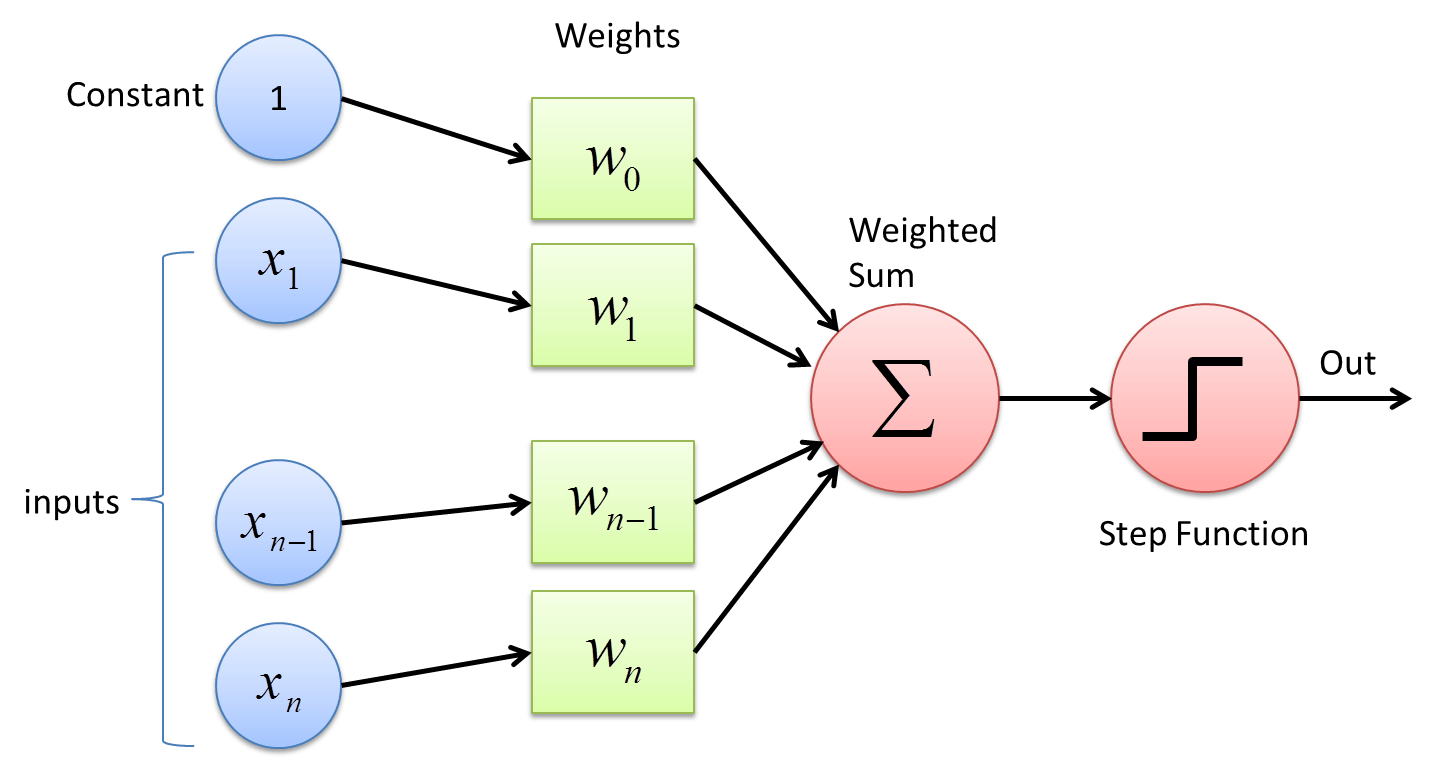
\includegraphics[width = 0.8\textwidth]{images/perceptron}
    \caption{Schematic picture of a single layer perceptron. The input vector is linearly combined with the bias factor and sent to an activation function to produce the numerical "binary" output.}
    \label{fig:perceptron}
\end{figure}

The most common architecture for a NN is the so-called \textit{feed-forward} architecture, where many individual perceptrons are arranged in chained layers, which take as input the output of previous layers along with a straight information flux. More complex architectures could implements also recursive connection, linking a layer to itself, but it should be regarded as sophistication to the standard case. There are endless possibilities of combination and arrangement of neurons inside a NN's layer, but the most simple ones are known as fully-connected layers, where every neuron is linked with each other neuron of the following layer, as shown in Figure \ref{fig:fully_connected}. Each connection has its weight, which contributes to modulate the overall combination of signals. The training of a NN consists then in the adjustment and fine-tuning of all the network's weights and parameters through iterative techniques until the desired precision in the output generation is reached.

\begin{figure}
    \centering
    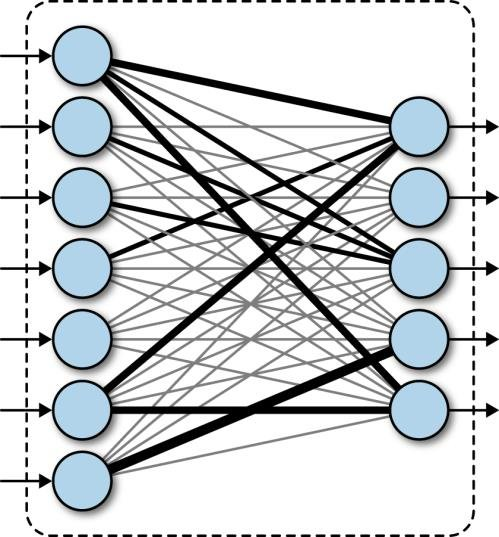
\includegraphics[width = 0.4\textwidth]{images/fully_connected}
    \caption{Schematic representation of a fully connected (or dense) layer. Every neuron from the first layer is connected with every output neuron. The link thickness represent the absolute value of the combination weight for that particular value. }
    \label{fig:fully_connected}
\end{figure}

Although a fully connected network represents the simplest linking choice, the insertion of each weight increases the number of overall parameters, and so the complexity of the model. Thus we want to create links between neurons smartly, rejecting the less useful ones. Depending on the type of data under analysis there are many different established typologies of layers. For example, in the image processing field, the most common choice is the convolutional layer, which implements a sort of discrete convolution on the input data, as shown in Figure \ref{fig:convolutional}. While processing images, the convolution operation confers to the perception of correlation between adjacent pixels of an image and their color channels, allowing a sort of spatial awareness. Furthermore, the majority of traditional computer vision techniques are based on the discrete convolution of images, and on the features extracted from them.

As a matter of principle a NN with just two successive layers, which is called a \textit{shallow} network, and with an arbitrary number of neurons per layer, can approximate arbitrary well any kind of smooth enough function \cite{pinkus_1999}. However, direct experience suggests that networks with multiple layers, called \textit{deep} networks, can reach equivalent results exploiting a lower number of parameters overall. This is the reason why this discipline goes under the name of \textit{deep} learning: it focuses on deep networks with up to tents of hidden layers. Such deep structures allow the computation of what is called deep features, so features of the features of the input data, that allows the network to easily manage concepts that would be bearly understandable for humans.

\begin{figure}
    \centering
    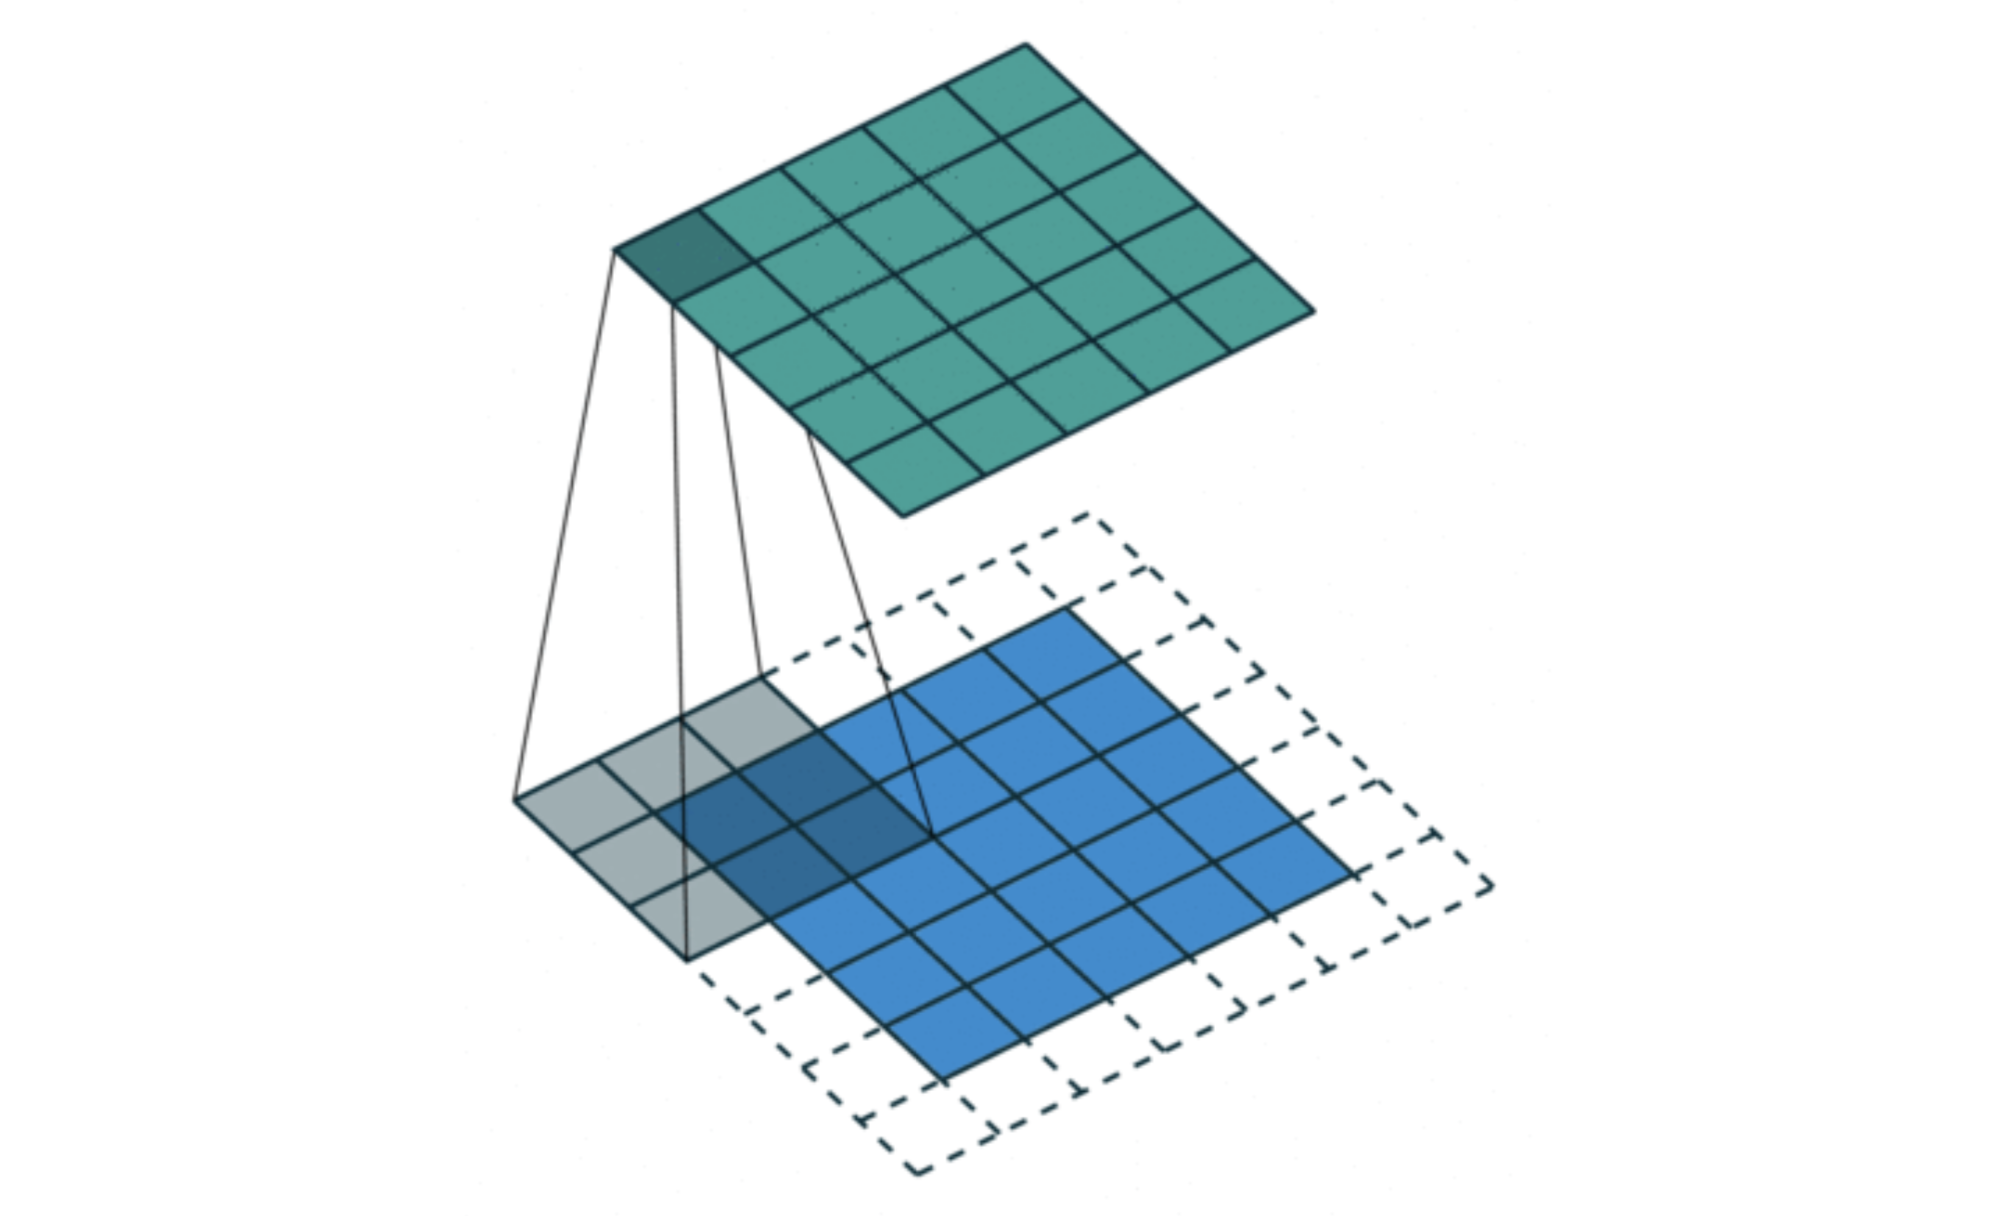
\includegraphics[width = 0.7\textwidth]{images/CL}
    \caption{Schematical representation of a convolutional layer. The input data are processed by a window kernel that slides all over the image. This operation can recreate almost all the traditional computer vision techniques, and can overcome them, creating new operations, which would be unthinkable to hand-engineered.}
    \label{fig:convolutional}
\end{figure}

\subsection{Training of a NN -  Error Back-Propagation}
Depending on the task the NN is designed for, it will have a different architecture and number of parameters. Those parameters are initialized to completely random values, tough. The training process is exactly the process of seeking iteratively the right values to assign to each parameter in the network in order to accomplish the task. The best start to understanding the training procedure is to look at how a supervised problem is solved. In supervised problems, we start with a series of examples of true connections between inputs and correspondent outputs and we try to generalize the rule behind those examples. After the rule has been picked up the final aim is to exploit it and to apply it to unknown data, so the new problem could be solved. In opposition to the concept of supervised problems, there are the \textit{unsupervised} problems, where the algorithm does not try to learn a rule from a practical example but try to devise it from scratch. A task typically posed as unsupervised is clustering, when different data are separated in groups based on the values of their features in the feature space. Usually, only the number of groups is taken in input from the algorithm, and the subdivision is completely performed by the machine. In the real world, by the way, there are many different and creative shapes between pure supervised and pure unsupervised learning, based on the actual availability of data and specific limitations to the individual task.

\begin{figure}
    \centering
    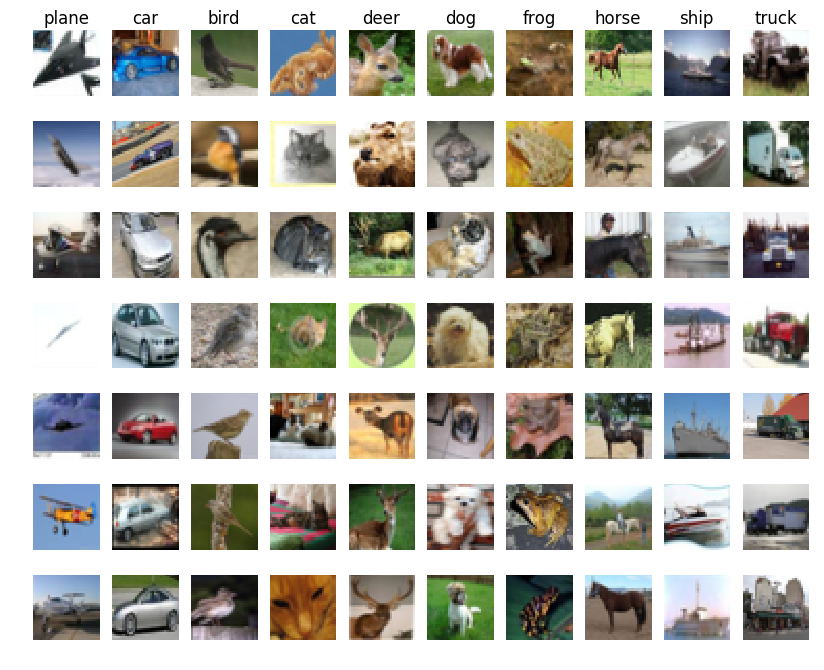
\includegraphics[width = 0.6\textwidth]{images/cifar10}
    \caption{Sample grid of images from the CIFAR10 dataset. Each one of the 32 $\times$ 32 image is labeled with one of the ten classes of objects: \textit{plane, car, bird, cat, deer, dog, frog, horse, ship, truck}.}
    \label{fig:cf10}
\end{figure}

A good example of supervised problems is the classification of images. Let's assume we have a whole dataset of pictures of different objects (as cats, dogs, cars, etc.) like the CIFAR10 \cite{cifar10} dataset. This famous dataset is made of over 60$K$ labeled colored images 32$\times$32 divided into 10 categories of objects as shown in Figure \ref{fig:cf10}. We could be interested in the creation of a NN able to assign at every image its belonging class. This NN could be arbitrarily complex but it certainly will take as input a 32$\times$32$\times$3 RGB image and the output will be the predicted class. A typical output for this problem would be a probability distribution over all the 10 classes like:

\begin{align}
    \vec p & = (p_1, p_2, \dots, p_{10}), \\
    &\sum_{i=1}^{10} p_i = 1,
\end{align}
and it should be compared with the true label, that is represented just as a binary sequence $\vec t$ with the bit correspondent to the belonging class set as 1, and all the others value set to 0:

\begin{equation}
    \vec t = (0,0,\dots, 1, \dots,0,0).
\end{equation}

Every time an image is given to the model an estimate of the output is produced. Thus, we need to measure the \textit{distance} between that prediction and the true value, to quantify the error made by the algorithm and try to improve the model's predictive power. The functions used for this purpose are called loss functions. The most common choice is the Mean Squared Error (MSE) function that is simply the averaged $L^2$ norm of the difference vector between $\vec p$ and $\vec t$:

\begin{equation}
    MSE = \frac{1}{n} \sum_{i=0}^{n} (t_i - p_i)^2.
    \label{eq:MSE}
\end{equation}

Let's say the NNunder training has $L$ consecutive layers, each one with its activation function $f^k$ and its weights vector $\vec w^k$, hence the prediction vector $\vec p$ could be seen as the result of the concesutive, nested, application through all the layers:

\begin{equation}
    \vec p = f^L(\vec w^L \cdot (f^{L-1}(\vec w^{L-1} \cdot ... \cdot f^1(\vec w^1 \cdot \vec x)))).
    \label{eq:neste_layers}
\end{equation}

From both equations \ref{eq:MSE} and \ref{eq:neste_layers} it is clear that the loss function could be seen as a function of all the weights vectors of every layer of the network. So if we want to reduce the distance between the NN prediction and the true value we need to modify those weights to minimize the loss function. The most established algorithm to do so for a supervised task in a feed-forward network is the so-called \textit{error back-propagation}. The back-propagation method is an iterative technique that works essentially computing the gradient of the loss function with respect to the weights using the derivative chain rule and updating by a small amount the value of each parameter to lower the overall loss function at each step. Each weight is  \textit{moved} counter-gradient, and summing all the contribution to every parameter the loss function approaches its minimum. In equation \ref{eq:weight_update} is represented the variation applied to the $j^{th}$ weight in the $i^{th}$ layer in a single step of the method:

\begin{equation}
    \Delta w_{ij} = - \eta \frac{\partial E}{\partial w_{ij}},
    \label{eq:weight_update}
\end{equation}
where $E$ is the error function, and $\eta$ is the \textit{learning coefficient}, that modulate the effect of learning through all the training process. This iterative procedure is applied completely to each image in the training set several times, each time the whole dataset is reprocessed is called an \textit{epoch}. The great majority of the dataset is exploited in the training phase to keep running this trial and error process and just a small portion is left out (typically 10\% of the data) for a final performance test.

The loss function shall inevitably be differentiable, and its behavior heavily influences the success of the training. If the loss function presents a gradient landscape rich of local minima the gradient descent process would probably get stuck in one of them. More sophisticated algorithms capable of avoiding this issue have been devised, with the insertion of some degree of randomness in them, as the Stochastic Gradient Descent algorithm, or the wide used \textit{Adam} optimizer \cite{1412.6980}.

The training phase is the pulsing heart of a DL model development and it could take even weeks on top-level computers for the most complicated networks. In fact, one of the great limits to the complexity of a network during the designing phase is exactly the available computational power. There are many more further technical details necessary for proper training, the adjustment of which can heavily impact the quality of the algorithm.

However, after the training phase, we need to test the performance of the NN. This is usually done running the trained algorithm on never seen before inputs (the test dataset) and comparing the prediction with the ground-truth value. A good way to evaluate the quality of the results is to use the same function used as the loss function during the training, but there is no technical restriction to the choice of this quality metric. The average score on the whole test set is then used as a numerical score for the network, and it allows straightforward comparison with other models' performances, trained for the same task.

All this training procedure is coherently customized to every different application, depending on which the problem is posed as supervised or not and depending on the more or less complex network's architecture. The leitmotif is always finding a suitable loss function that quantifies how well the network does what it has been designed to do and trying to minimize it, operating on the parameters that define the network structure.

    \clearpage
    \section{Deep Learning-Based Segmentation Algorithms} \label{ssec:segmentation}
In digital image processing, image segmentation is the process of recognizing and subdividing an image into different regions of pixels that show similar features, like color, texture, or intensity. Typically, the task of segmentation is to recognize the edges and boundaries of the different objects in the image and assigning a different label to every detected region. The result of the segmentation process is an image with the same dimensions of the starting one made of solid color regions, representing the detected objects. This image is called \textit{segmentation mask}. In Figure \ref{fig:seg_example} is shown an example of segmentation of a picture of an urban landscape: different colors are linked to different classes of objects like persons in magenta and scooters in blue. This technology has a significant role in a wide variety of application fields such as scene understanding, medical image analysis, augmented reality, etc.

\begin{figure}
    \centering
    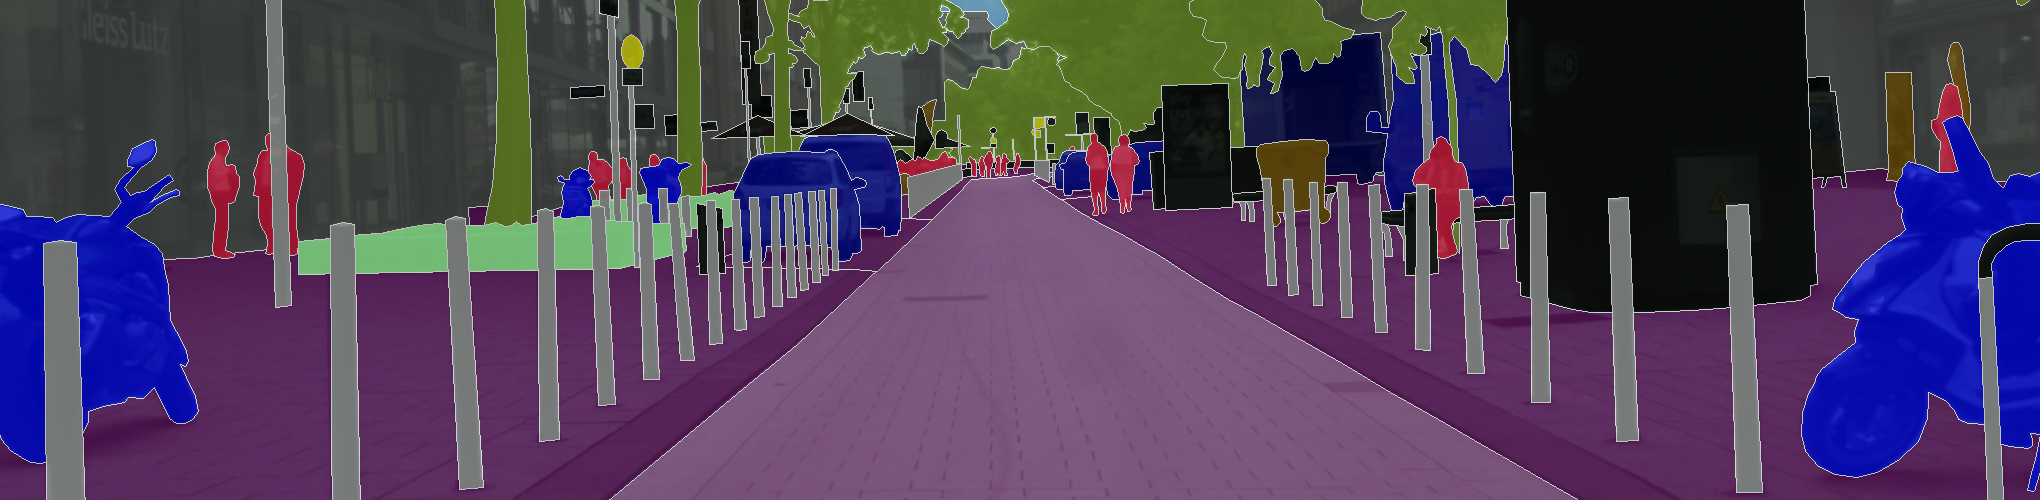
\includegraphics[width = \textwidth]{images/seg_example}
    \caption{Example of the resulting segmentation mask of an image of an urban landscape. Every interesting object of the image is detected and a solid color region replaces it in the segmentation mask. Every color corresponds to a different class of objects, for example, persons are highlighted in magenta and scooters in blue. The shape and the boundaries of every region should match as precisely as possible the edges of the objects.}
    \label{fig:seg_example}
\end{figure}

A relatively easy segmentation problem, and one of the first to be tackled, could be distinguishing an object from the background in a grey-scale image. The easiest technique to perform segmentation in this kind of problem is based on thresholding. Thresholding is a binarization technique based on the image's grey-level histogram: to every pixel with luminosity above that threshold is assigned the color \textit{white}, and vice versa the color \textit{black}. However, this is a very primitive and fallacious, yet very fast method, and it manages poorly complex images or images with un-uniformity in the background.

A lot of other traditional techniques improve this first segmentation method \cite{Chouhan2018}. Some are based on the object's edges recognition, exploiting the sharp change in luminosity typically in correspondence of the boundary of a shape. Other techniques exploit instead a region-growing technology, according to which some \textit{seed} region markers are scattered on the image, and the regions corresponding to the objects in the image are grown to incorporate adjacent pixels with similar properties.

\begin{figure}
    \centering
    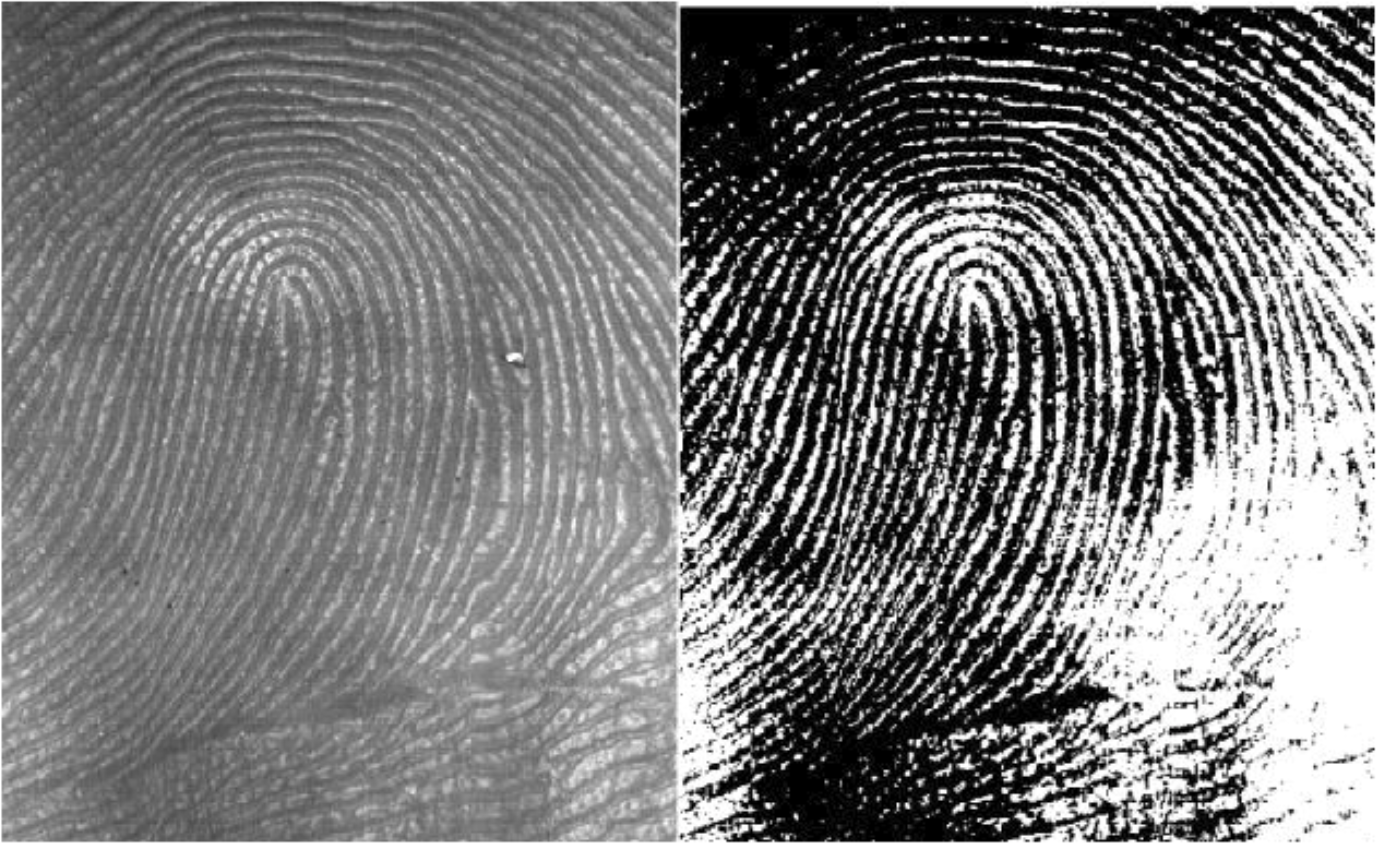
\includegraphics[width = 0.7\textwidth]{images/fingerprints}
    \caption{Example of the resulting segmentation mask of an image of a fingeprint obtained trhough a thresholding algorithm. The result is not extremely good, but this techinque is very easy to implement and runs very quickly.}
    \label{fig:fing_prints}
\end{figure}

\subsection{State of the Art on Deep Learning Segmentation} \label{ssec:soa_seg}
Similarly to many other traditional tasks, also for segmentation, there has been a thriving development lead by the diffusion of deep learning, that boosted the performances resulting in what many regards as
a paradigm shift in the field \cite{deep_seg_SOA}.

In further detail, image segmentation can be formulated as a classification problem of pixels with semantic labels (semantic segmentation) or partitioning of individual objects (instance segmentation). Semantic segmentation performs pixel-level labeling with a set of object categories (e.g. boat, car, person, tree) for all the pixels in the image, hence it is typically a harder task than image classification, which requires just a single label for the whole image. Instance segmentation extends semantic segmentation scope further by detecting and delineating each object of interest in the image (e.g. partitioning of individual nuclei in a histological image).

There are many prominent Neural Network architectures used in the computer vision community nowadays, based on very different ideas such as convolution, recursion, dimensionality reduction, and image generation. This section will provide an overview of the state of the art of this technology and will dwell briefly on the details behind some of those innovative architectures.

\begin{description}
    \item [Recurrent Neural Networks (RNNs) and the LSTM] \hfill \\
        The typical application for RNN is processing sequential data, as written text, speech or video clips, or any other kind of time-series signal. In this kind of data, there is a strong dependency between values at a given time/position and values previously processed. Those models try to implement the concept of \textit{memory} weaving connections, outside the main information flow of the network, with the previous NN's input. At each time-stamp, the model collects the input from the current time $X_i$ and the hidden state from the previous step $h_{i-1}$ and outputs a target value and a new hidden state (Figure \ref{fig:recNN}). Typically RNN cannot manage easily long-term dependencies in long sequences of signals. There is no theoretical limitation in this direction, but often it arises vanishing (or exploding) gradient problematics during the training phase. A specific type of RNN has been designed to avoid this situation, the so-called Long Short Term Memory (LSTM) \cite{LSTM}. The LSTM architecture includes three gates (input gate, output gate, forget gate), which regulate the flow of information into and out from a memory cell, which stores values over arbitrary time intervals.

        \begin{figure}
            \centering
            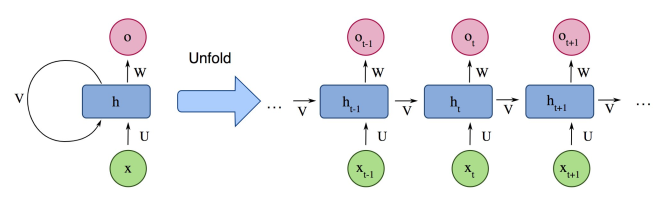
\includegraphics[width = 0.8\textwidth]{images/recNN}
            \caption{Example of the structure of a simple Recurrent Neural Network from  \cite{deep_seg_SOA}.}
            \label{fig:recNN}
        \end{figure}

    \item [Encoder-Decoder and Auto-Encoder Models] \hfill \\
        Encoder-Decoder models try to learn the relation between an input and the corresponding output with a two steps process. The first step is the so-called \textit{encoding} process, in which the input $x$ is compressed in what is called the \textit{latent-space} representation $z = f(x)$. The second step is the \textit{decoding} process, where the NN predicts the output starting from the latent-space representation $ y = g(z)$. The idea underneath this approach is to capture in the latent-space representation the underlying semantic information of the input that is useful for predicting the output. ED models are widely used in image-to-image problems (where both input and output are images) and for sequential-data processing (like Natural Language Processing, NLP). In Figure \ref{fig:EDNN} is shown a schematic representation of this architecture. Usually, these model follow a supervised training, trying to reduce the reconstruction loss between the predicted output and the ground-truth output provided while training. Typical applications for this technology are image-enhancing techniques like de-noising or super-resolution, where the output image is an improved version of the input image. Or image generation problems (e.g. plausible new human faces generation) in which all the properties which define the type of image under analysis should be learned in the representation latent space.

        \begin{figure}
            \centering
            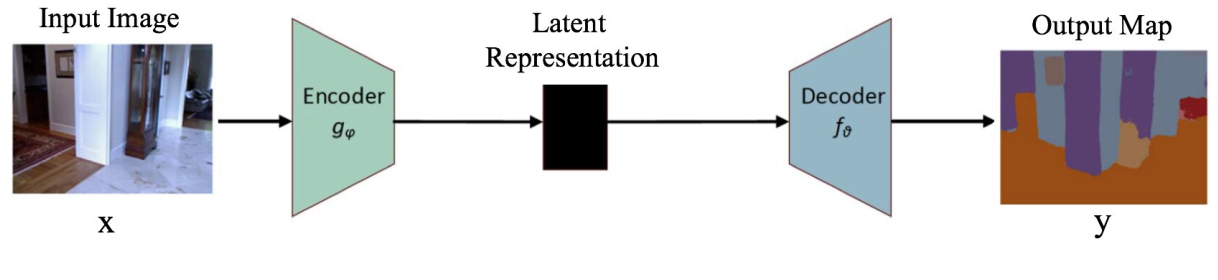
\includegraphics[width = 0.8\textwidth]{images/EDnet}
            \caption{Example of the structure of a simple Encoder-Decoder Neural Network from  \cite{deep_seg_SOA}.}
            \label{fig:EDNN}
        \end{figure}

    \item [Generative Adversarial Networks (GANs)] \hfill \\
        The peculiarity of Generative Adversarial Network (GAN) lies in its structure. It is actually made of two distinct and independent modules: a generator and a discriminator, as shown in Figure \ref{fig:GAN}. The first module $G$, responsible for the generation, typically learns to map a prior random distribution of input $z$ to a target distribution $y$, as similar as possible to the target $G = z \rightarrow y$ (i.e. almost any kind of image-to-image problem could be addressed with GANs, as in \cite{1611.07004}). The second module, the discriminator $D$, instead is trained to distinguish between \textit{real} and \textit{fake} images of the target category. These two networks are trained alternately in the same training process. The generator tries to fool the discriminator and vice versa. The name adversarial is actually due to this \textit{competition} within different parts of the network. The formal manner to set up this adversarial training lies in the accurate choice of a suitable loss function, that will look like: $$L_{GAN} = \mathbb{E}_{x \sim p_{data}(x)}[logD(x)] + \mathbb{E}_{z \sim p_{z}(z)}[log(1-D(G(z)))]$$.
        The GAN is thus based on a min-max game between $G$ and $D$. $D$ aims to reduce the classification error in distinguishing fake samples from real ones, and as a consequence maximizing the $L_{GAN}$. On the other hand, $G$ wants to maximize the $D$'s error, hence minimizing $L_{GAN}$. The result of the training process is the trained generator $G^*$, capable of produce an arbitrary number of new data (images, text, or whatever else): $$ G^* = \operatorname*{arg\,min_Gmax_D} L_{GAN}$$.
        This peculiar architecture has yielded several interesting results and it has been developed in many different directions, with influences and contaminations with other architectures \cite{1611.07004}.

        \begin{figure}
            \centering
            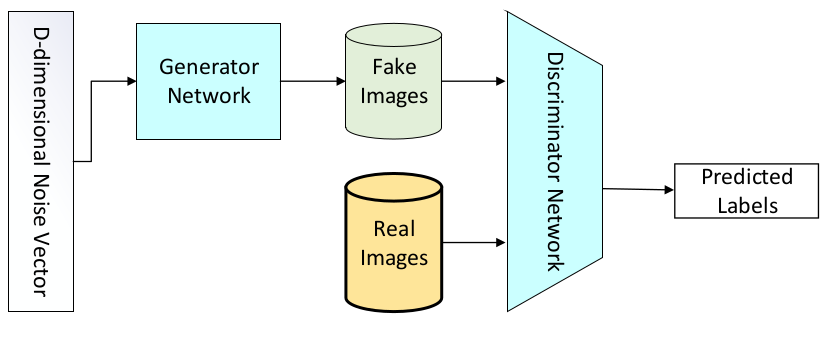
\includegraphics[width = 0.6\textwidth]{images/GAN}
            \caption{Schematical representation of a Generative Adversarial Networks, form \cite{deep_seg_SOA}.}
            \label{fig:GAN}
        \end{figure}

    \item [Convolutional Neural Networks (CNNs)] \hfill \\
        As stated before CNNs are a staple choice in image processing DL applications. They mainly consist of three types of layers:

        \begin{enumerate}[i]
            \item convolutional layers, where a kernel window of parameters is convolved with the image pixels and produce numerical features maps.

            \item nonlinear layers, which apply an activation function on feature maps (usually element-wise). This step allows the network to introduce non-linear behavior and then increasing its modeling capabilities.

            \item pooling layers, which replace a small neighborhood of a feature map with some statistical information (mean, max, etc.) about the neighborhood and reduce the spatial resolution.
        \end{enumerate}

        Given the arrangement of successive layers, each unit receives weighted inputs from a small neighborhood, known as the receptive field, of units in the previous layer. The stack of layers allows the NN to perceive different resolutions: the higher-level layers learn features from increasingly wider receptive fields. The leading computational advantage given by CNN architecture lies in the sharing of kernels' weights within a convolutional layer. The result is a significantly smaller number of parameters than fully-connected neural networks. In section \ref{ssec:sttrNN} will be shown a particular application of this architecture, known as \textit{style-transfer} network, which is a particular algorithm capable of implanting the visual texture of a \textit{style} image onto the content of a different image, producing interesting hybrid images. Some of the most notorious CNN architectures include: AlexNet \cite{AlexNet}, VGGNet \cite{1409.1556}, and U-Net \cite{U-net}.
\end{description}

For this work, U-net architecture is particularly interesting. The U-net model was initially developed for biomedical image segmentation, and in its structure reflects characteristics of both CNN and Encoder-Decoder models. Ronneberger et al.\cite{U-net} proposed this model for segmenting biological microscopy images in 2015. The U-Net architecture is made of two branches, a contracting path to capture context, and a symmetric expanding path (see Figure \ref{fig:unet}). The down-sampling flow is made of a Fully Convolutional Network (FCN)-like architecture that computes features with 3 $\times$ 3 kernel convolutions. On the other hand, the up-sampling branch exploits up-convolution operations (or deconvolution), reducing the number of feature maps while increasing their dimensions. Another characteristic of this architecture is the presence of direct connections between layers of a similar level of compression in compressing and decompressing branches. Those links allow the NN to preserve spatial and pattern information. The Network flow eventually ends with a 1 $\times$ 1 convolution layer responsible for the generation of the segmentation mask of the input image.

    \begin{figure}
        \centering
        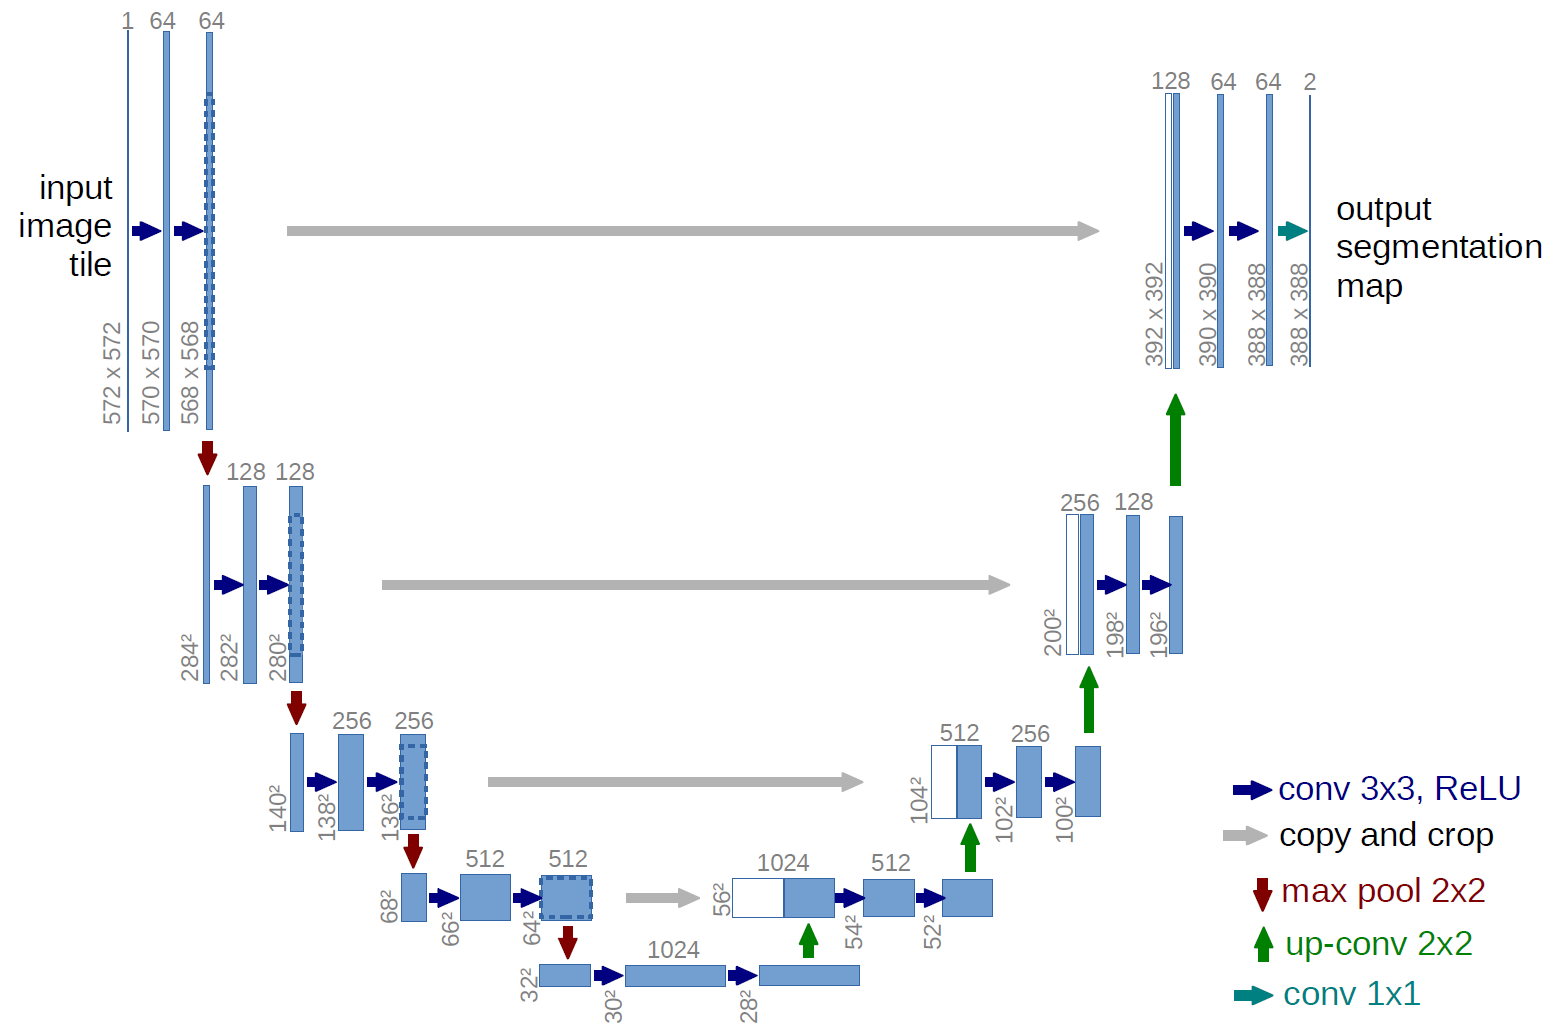
\includegraphics[width = 0.8\textwidth]{images/unet}
        \caption{Scheme of the typical architecture of a U-net NN. This particular model was firstly proposed by Ronneberger \textit{et al.} in \cite{U-net}.}
        \label{fig:unet}
    \end{figure}

\hl{I SHOULD REPORT HERE SOME ACTUAL RESULT OF SEGMENTATION OF HISTOLOGICAL SEGMENTATION TO CONCLUDE THE DISCUSSION. NUCLEI DETECTION OR SIMILA.}

    \begin{figure}
        \centering
        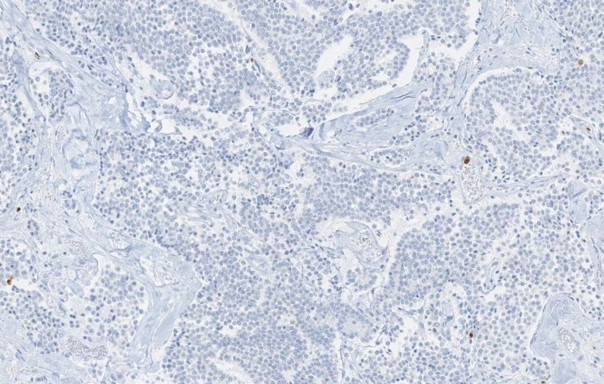
\includegraphics[width = 0.4\textwidth]{images/PancTissue}
        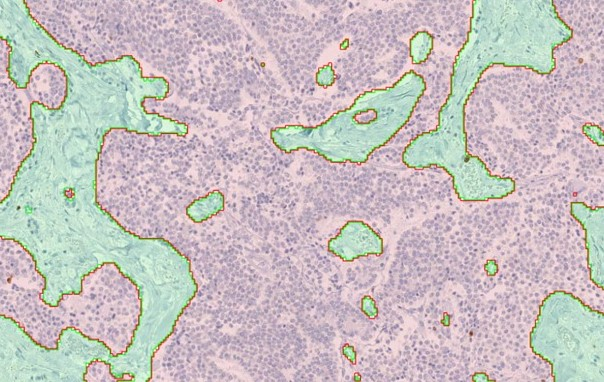
\includegraphics[width = 0.4\textwidth]{images/PancTissueSeg}
        \caption{}
        \label{fig:autom_seg}
    \end{figure}

\subsection{Image Segmentation Datasets}
Besides the choice of suitable architecture the most important aspect while developing a NN is the dataset on which perform the training process. Let's confine the discussion only to image-to-image problems, like segmentation problems. There are a lot of widely used datasets, but I want to mention just a few of them to give the idea of their typical characteristics.

A good example of segmentation is the Cityscapes dataset \cite{Cityscapes}, which is a large-scale database with a focus on semantic understanding of urban street scenes. The dataset is made of video sequences from the point of view of a car in the road traffic, from 50 different cities in the world. The clips are made of 5K frames, labeled with extremely high quality at pixel-level and an additional set of 20K weakly-annotated frames. Each pixel in the segmentation mask contains the semantic classification, among over 30 classes of objects. An example of an image from this dataset is shown in Figure \ref{fig:seg_example}.

The PASCAL Visual Object Classes (VOC) \cite{PASCAL} is another of the most popular datasets in computer vision. This dataset is designed to support the training of algorithms for 5 different tasks: segmentation, classification, detection, person layout, and action recognition. In particular, for segmentation, there are over 20 classes of labeled objects (e.g. planes, bus, car, sofa, TV, dogs, person, etc.). The dataset comes divided into two portions: training and validation, with 1,464 and 1,449 images, respectively. In Figure \ref{fig:PASCAL} is shown an example of an image and its corresponding segmentation mask.

    \begin{figure}
        \centering
        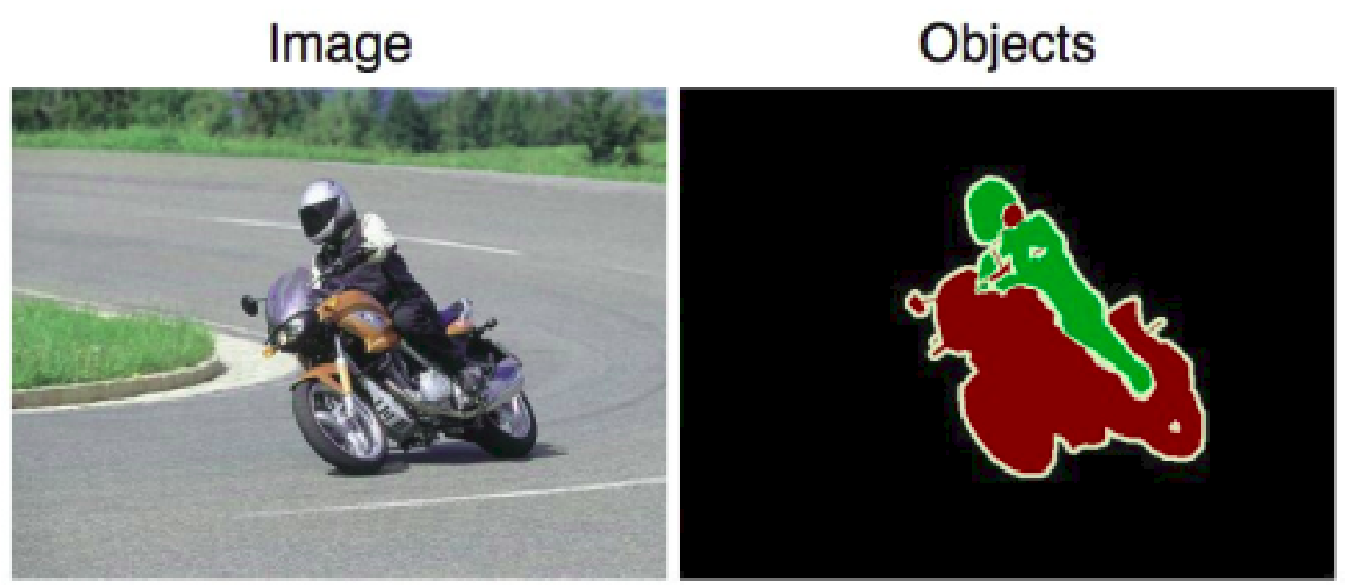
\includegraphics[width = 0.5\textwidth]{images/PASCAL}
        \caption{An example image from the PASCAL dataset and its corresponding segmentation mask \cite{PASCAL}.}
        \label{fig:PASCAL}
    \end{figure}

It is worth mentioning that in the medical image processing domain typically the available dataset is definitely not that rich and vast (that is actually the seed of this work) and thus many techniques of data augmentation have been devised, to get the best out of the restricted amount of material. Generally, data augmentation manipulates the starting material applying a set of transformation to create new material, like rotation, reflection, scaling, cropping and shifting, etc. Data augmentation has been proven to improve the efficacy of the training, making the model less prone to over-fitting, increasing the generalization power of the model, and helping the convergence to a stable solution during the training process.

    \clearpage

\chapter{Technical Tools for Model Development} \label{sec:tech_tool}
    As mentioned in the introduction, this project wants to produce synthetic histological images paired with their corresponding segmentation mask, to train Neural Networks for the automatization of real histological images analysis. The production of artificial images passes through the processing of a three-dimensional, virtual model of a histological structure, which is the heart of this thesis work. The detailed description of the development of the two proposed histological models will follow the present chapter and will occupy the entire chapter \ref{sec:models}. Here I will dwell, instead, on every technical tool employed during the models' designing phase. From the practical point of view, this project is quite articulated and the development has required the harmonization of many different technologies, tools, and code libraries. The current chapter should be seen as a theoretical complement for chapter \ref{sec:models}, and its reading is suggested to the reader for any theoretical gap or for any further technical deepening. The reader already familiar with those technical tools should freely jump to the models' description.

All the code necessary for the work has been written in a pure \texttt{Python} environment, using several already established libraries and writing by myself the missing code for some specific applications. I decided to code in \texttt{Python} given the thriving variety of available libraries geared toward scientific computation, image processing, data analysis, and last but not least for its ease of use (compared to other programming languages). In each one of the following subsections, I will mention the specific code libraries which have been employed in this project for every technical necessity.

    \section{Materials and Tools for the Development}
Before delving into the details of the development of the two histological models, which are the heart of this work, it should be convenient to dwell on every tool employed during the design phase.

All the work has been done in a pure Python environment, using several already established libraries and writing on my own the missing code, for some specific applications. All the code written during the development, the images and the data produced have been collected in a devoted repository on GitHub \cite{repo}. I decided to code in Python given the thriving variety of available libraries geared toward scientific computation, image processing , data analysys and last but not least for its ease of use (compared to other programming languages).

In this section it will follow a description, in no particular order, of the less common tools I used during my work.

\subsection{Quaternions}
Quaternions are, in mathematics, a number system that expands in four dimensions the complex numbers. They have been described for the first time by the famous mathematician William Rowan Hamilton in 1843. This number system define three independent \textit{imaginary} units $\bm{i}$, $\bm{j}$, $\bm{k}$ as in (\ref{eq:quat_rules}), which allows the general representation of a quaternion $\bm{q}$ is (\ref{eq:quat}) and its inverse $\bm{q}^{-1}$ (\ref{eq:inv_quat}) where $a,b,c,d$ are real numbers:

\begin{align}
    \bm{i}^2 & = \bm{j}^2 = \bm{k}^2 = \bm{i}\bm{j}\bm{k} = -1, \label{eq:quat_rules}\\
    \bm{q} & = a + b\bm{i} + c\bm{j} + d\bm{k}, \label{eq:quat}\\
    \bm{q}^{-1 } = (a + b\bm{i} + c\bm{j} + d\bm{k})^{-1} & = \frac{1}{a^2 + b^2 + c^2 +d^2}\ (a - b\bm{i} - c\bm{j} - d\bm{k}). \label{eq:inv_quat}
\end{align}

Furthermore, the multiplication operation between quaternionn does not benefit from commutativity, hence the product between basis elements will behave as follows:

\begin{align}
    \bm{i} \cdot 1 = 1 \cdot \bm{i} = \bm{i}, & \qquad  \bm{j} \cdot 1 = 1 \cdot \bm{j} = \bm{j}, \qquad \bm{k} \cdot 1 = 1 \cdot \bm{k} = \bm{k} \label{eq:Ham_prod}\\
    & \bm{i} \cdot \bm{j}= \bm{k}, \qquad \bm{j} \cdot \bm{i}= -\bm{k} \nonumber \\
    & \bm{k} \cdot \bm{i}= \bm{j}, \qquad \bm{i} \cdot \bm{k}= -\bm{j} \nonumber \\
    & \bm{j} \cdot \bm{k}= \bm{i}, \qquad \bm{k} \cdot \bm{j}= -\bm{i}. \nonumber
\end{align}

This number system has plenty of peculiar properties and application, but for the purpose of this project quaternions are important for their ability of representing in a very convenient way rotations in three dimensions. In fact, the particular subset of quaternions with vanishing real part ($a=0$) has a useful, yet redundant, correspondence with the group of rotations in tridimensional space. Every 3D rotation of an object can be represent by a 3D vector $\vec u$: the vector's direction indicates the axis of rotation and the vector magnitude $|\vec u|$ express the angular extent of rotation. However, the matricial operation which express the rotation around an arbitrary vector $\vec u$ it is quite complex and does not scale easily for multiple rotations \cite{10.1007/BFb0031048}, which brings to very heavy and entangled computations.

Using quaternions for expressing rotations in space, instead, it is very convinient. Given the unit rotation vector $\vec u$ and the rotation angle $\theta$, the corresponding rotation quaternion $\bm{q}$ becomes (\ref{eq:rot_quat}):
\begin{align}
    \vec u & = (u_x, u_y, u_z) = u_x\bm{i} + u_y\bm{j} + u_z\bm{k}, \\
    \bm{q} & = e^{\frac{\theta}{2}(u_x\bm{i} + u_y\bm{j} + u_z\bm{k})} = \cos{\frac{\theta}{2}} + (u_x\bm{i} + u_y\bm{j} + u_z\bm{k})\sin{\frac{\theta}{2}}, \label{eq:rot_quat}\\
    \bm{q}^{-1} & = \cos{\frac{\theta}{2}} - (u_x\bm{i} + u_y\bm{j} + u_z\bm{k})\sin{\frac{\theta}{2}},
\end{align}
where in (\ref{eq:rot_quat}) we can clearly see a generalization of the Euler's formula for the exponential notation of complex numbers, which hold for quaternions. It can be shown that the application of the rotation represented by $\bm{q}$ on an arbitrary 3D vector $\vec v$ should be easily expressed as:
\begin{equation}
    \vec v\,' = \bm{q} \vec v \bm{q}^{-1},
\end{equation}
using the Hamilton product defined on quaternions (\ref{eq:Ham_prod}). This rule raises a very convinient and an extremily scalable way to compute consecutive rotations in space. Given two independent and consecutive rotations represented by the two quaternions $\bm{q}$ and $\bm{p}$ applyed on the vector $\vec v$ the resulting rotated vector $\vec v\,'$ is simply yielded as:
\begin{equation}
    \vec v\,' = \bm{p} ( \bm{q} \vec v \bm{q}^{-1} ) \bm{p}^{-1} = (\bm{p}\bm{q}) \vec v (\bm{q}\bm{p})^{-1},
\end{equation}
which essentially is the application of the rotation $\bm{r} = \bm{q}\bm{p}$ on the vector $\vec v$. This representation is completely coherent with the algebra of 3D rotations, which does not benefit from commutativity in turn.

Given this convinient property, quaternions are in deed widely used in all sort of application of digital 3D space design, as for simulations and for videogame design. The position of an object in the space in simulations is generally given by the application of several independent rotations, typically in the order of tenth of rotations, which with quaternions is given easily by the product of simple objects. Every other alternative method would imply the use of matricial representation of rotations or other rotation systems as Euler's anglse and would eventually make the computation prohibitive.

The use of quaternions in this work will be justified in section \ref{ssec:Lsys} and [??], while speaking of parametric L-systems in 3D space, used to build the backbone of the ramificated structure of blood vassels in the reconstruction of a sample of pancreatic tissue.

\subsection{Parametric L-Systems} \label{ssec:Lsys}

\subsection{Voronoi Tassellation}

\subsection{Saltelli Algorithm - Randon Number Generation}

\subsection{Planar Section of a Polyhedron}

\subsection{VPython - 3D Visualization}

\subsection{SnakeMake}

\subsection{Perlin Noise}

\subsection{Style-Transfer Neural Network}\label{ssec:sttrNN}

    \clearpage

\chapter{Tissues Model Development} \label{sec:models}
    The main goal of the present work, as stated before, is to recreate a three-dimensional virtual model of histological tissue as faithfully as possible and then, to perform planar sectioning on it to emulate virtually the traditional histological specimen preparation procedure. The creation of a model of such complex structures is definitely a high-level problem, and it has required a careful designing, made of subsequent stages of improvements. 
In section \ref{ssec:panc_tis_mod}, I will describe all the necessary steps to create the model of a small region of pancreatic tissue, while in section \ref{ssec:derm_tis_mod} I will expose the steps I followed to build a model of dermal tissue. In section \ref{sec:synth_image}, instead, I will show the resulting synthetic images from the sectioning process performed on both the models and all the enrichments and processing necessary to give them the most realistic look I was able to recreate.

    \section{Model Development}
The main goal of the present work, as stated before, is to recreate a three-dimensional virtual model of histological tissue as faithfully as possible and then, to perform planar sectioning on it to emulate virtually the traditional histological specimen preparation procedure. The creation of a model of such complex structures is definitely a high-level problem, and it has required a careful designing, made of subsequent stages of improvements. In this work, I will report only two specific attempts of modelization: the first aiming to represent pancreatic tissue, and the second oriented toward dermal tissue.

\begin{figure}[b!]
    \centering
    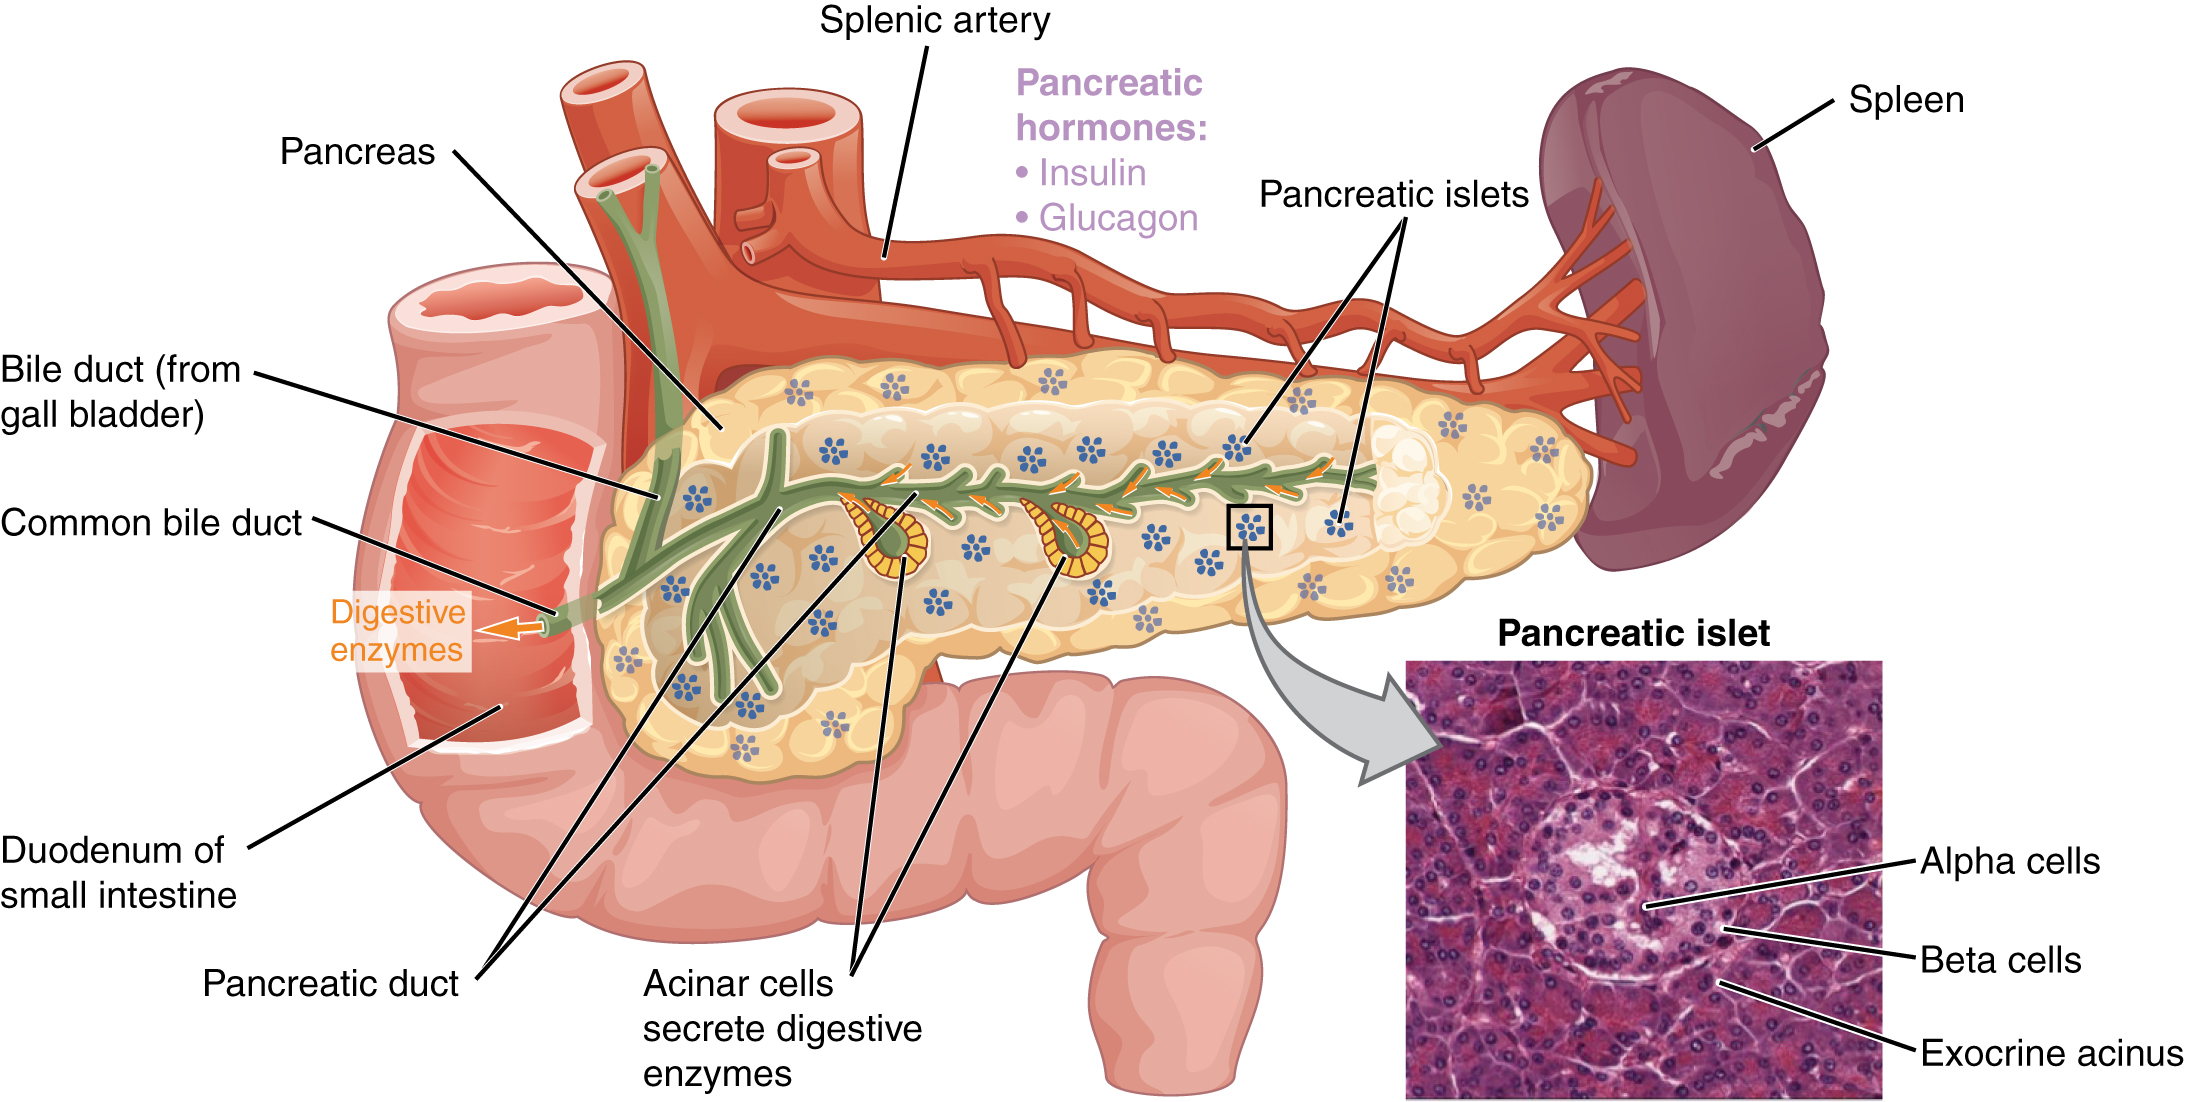
\includegraphics[width = 0.6\textwidth]{images/panc_struct}
    \caption{A picture of pancreas' structure in its phisiologiacl context. In this picture is clearly visible the macroscopic structure and the galndular organization at microscopic level, and how it reflects in the histological sample.}
    \label{fig:panc_struct}
\end{figure}

\subsection{Pancreatic Tissue Model} \label{ssec:panc_tis_mod}
The Pancreas is an internal organ of the human body, part of both the digestive system and the endocrine system. It acts as a gland with both endocrine and exocrine functions, and it is located in the abdomen behind the stomach. Its main endocrine duty is the regulation of sugar levels in the blood and the secretion of hormones, like insulin and glucagon. While, as a part of the digestive system it acts as an exocrine gland secreting pancreatic juice. The majority of pancreatic tissue has a digestive role, and the cells with this role form clusters (\textit{acini}) around the small pancreatic ducts, and are arranged in lobes. The acinus secrete inactive digestive enzymes called zymogens into the small intercalated ducts which they surround, and then in the pancreatic blood vessels system \cite{Pancreas}. In Figure \ref{fig:panc_struct} is shown a picture of the pancreas, with its structure and its placement in the human body.

All the tissue is actually rich in other important elements as the islets of Langerhans, and sporadic connective tissue all over the structure, which are clearly visible in the traditional histological specimens. In this first attempt of modelization from scratch this second layer of complexity has not been already considered, and the main focus has been to reflect only the main structural features on the virtual specimens. Given pancreatic tissue's organization the first features I decided to put emphasis on were: 1) The iterative (with a fractal-like behavior) ramification of blood vessels for the irrigation of glandular acinus, 2) The space-filling distribution of acinus in the tissue, in fact, we expect a homogeneous density in the organ and to not see \textit{holes} at all inside it. In this section I will describe step by step all the process I followed to create the model of a portion of pancreatic tissue, and all the interesting pitfalls I overcame.

% To make enumerated description:
\newcounter{mycounter}
\newcommand*{\mycount}{\stepcounter{mycounter}\themycounter}

\begin{description}
    \item [\mycount) 2D Ramification] \hfill \\
    The first step was took in two dimensions, and it was the choice of the right \textit{structure} to emulate the ramification of blood vessels in pancreatic tissue. The choice fell on a particular parametric L-system, as the one shown in Figure \ref{fig:bf_ls}, in section \ref{sec:tech_tool}. This structure is made of an iterative bifurcation of gradually shorter segments, with an angle of $\pm 85 \degree$ respect the main direction. For a start I added some features to give a more realistic look to the structure, which are all well represented in Figure \ref{fig:ram_feat}:

    \begin{figure}
        \centering
        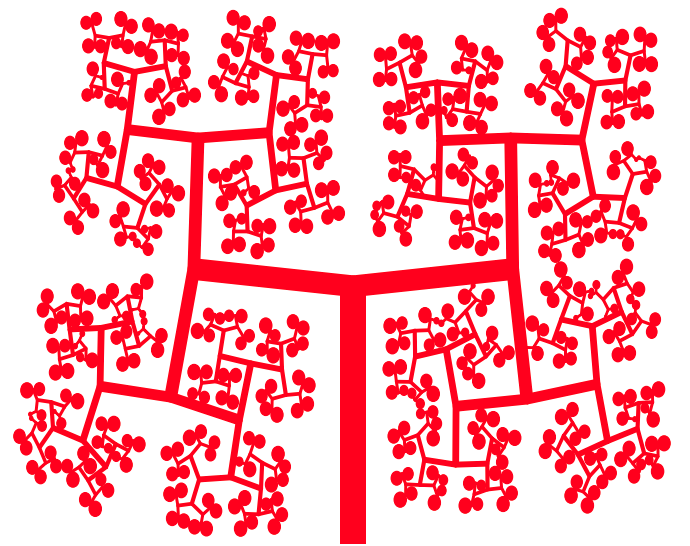
\includegraphics[width = 0.6\textwidth]{images/ram_feat}
        \caption{The development of the simple curve in Figure \ref{fig:bf_ls}, with some features to give it a more realistic look, like progressive thickness, angular noise in bifurcation and spheres at free ends of the ramification. The image is made using the tools exposed in section \ref{ssec:Lsys}.}
        \label{fig:ram_feat}
    \end{figure}

    \begin{itemize}
        \item A progressive thickness of the bifurcation's segments, starting from a thick main branch that dwindles every junction. The idea is that the main blood vessel becomes gradually smaller becoming capillaries for single-cell irrigation.
        \item A progressive randomness in the angular deflection at every fork. Perfectly repeated angles are almost nonexistent in nature, so I decided to introduce an increasing indetermination in the angle of bifurcation from the main branch to the free ends of the structure'branches.
        \item Spheres at the ends of each branch, which acts as glandular acini. The maximum radius is comparable to the length of the final segments.
        \item A mechanism to avoid self-superimposition between branches and spheres. After the insertion of noise, the cumulative effect on the final segments might lead to different branches to intersect. This is clearly a paradoxical situation, as real tissues while growing naturally occupy the space in a gradual way.
    \end{itemize}

    To produce the specific image in Figure \ref{fig:ram_feat} I used a particular setting of the tools described in section \ref{ssec:Lsys}, which have a greatly wider range of customization and could be used to create many other different structures to the need.

    \item [\mycount) Expansion to 3D] \hfill \\
    The successive step I followed was to expand this structure in three dimensions and fill the space in each of the three directions. The idea to evolve the structure in Figure \ref{fig:ram_feat} is simply to twist of 90$\degree$ the ramification at every junction point, in such a way to exit the previous belonging plane. However, putting into practice this development has not been easy. The organization of the structure in a 3D space requires an appropriate system of reference for handling subsequent rotations in three dimensions. The best option for handling relative 3D rotations, often used in computer graphics and every kind of 3D modelization, are quaternions, as shown in section \ref{ssec:quat}.

    \begin{figure}
        \centering
        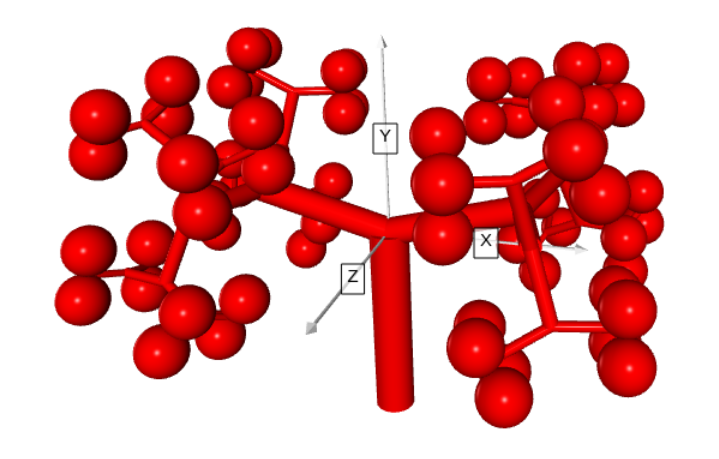
\includegraphics[width = 0.6\textwidth]{images/3d_ram}
        \caption{The three-dimensional expansion of the 2D ramification in Figure \ref{fig:ram_feat}.}
        \label{fig:3d_ram}
    \end{figure}

    In this new structure, segments are replaced with cylinders, and circles are replaced with spheres. At every bifurcation to every cylinder are applied the following transformations:
    \begin{itemize}
        \item a contraction in its extensions, regulated by an adjustable parameter $R$.
        \item the usual deviation of $\pm 85 \degree$ respect to the direction of the parent branch.
        \item a 90$\degree$ specific rotation along the axis of its parent branch.
    \end{itemize}

    The result of this procedure is a 3D ramification like the one in Figure \ref{fig:3d_ram}, in which we can recognize a good coverage of the space defined by the structure's boundaries and immediate relation with the 2D structure in Figure \ref{fig:ram_feat}. It should be noted that, in the further refinements of the model from now on, there won't be present the progressive angular indetermination on the direction of branches. Although it is a feature already implemented and working, it requires efficient control to avoid reciprocal overlapping between elements to produce a realistic structure. This second element has not been already developed and it would certainly enrich the representative power of the model.

    As for the 2D ramification the production of this structure has required the implementation of a tool for the 3D generation with a greatly wider power, able to produce almost any type of three-dimensional iterative structure after the right adjustment, and with a high degree of customization. It is necessary to mention the fundamental tool which allowed me to accomplish this step of the development, which is the \texttt{Python} library \texttt{VPython}: a library for 3D graphics visualization. This library allows a convenient and powerful interface to draw many types of objects and to move them around in space, which has been priceless to orient my self in three dimensions while developing the model and to produce all the 3D images visible in this work.

    \item [\mycount) Subdivision in Cells] \hfill \\
    Once the 3D backbone of the pancreatic tissue blood vessels ramification system has taken shape, the next step was to embed all this structure in a spatial partitioning process, to create the subdivision into single cells. To perform this important task I used a 3D Voronoi decomposition, as shown in section \ref{ssec:vor_tass}. Depending on the choice of the starting points, the Voronoi tessellation could be an excellent item to recreate individual cells because it could guarantee some important properties: all the regions are convex, adjacent, with similar size and volume, with different shapes, and without holes. These have been chosen as the most significant properties to be reflected in the first modelization of cells.

    As shown in section \ref{ssec:vor_tass}, the decomposition strongly depends on the choice of the starting point. Points spread uniformly on a 3D regular lattice will produce a series of parallelepipeds repeated in the space. An example of uniform tessellation is shown in Figure \ref{fig:reg_vor}. On the other side, a decomposition based on a quasi-random generated point can present all the good properties we mentioned before, including the diversity in shapes. In Figure \ref{fig:sal_vor} is shown an example of a Voronoi decomposition based on points sampled in a 3D with the Saltelli algorithm, in reference to section \ref{ssec:saltelli}. Regardless of the points sampling technique, the boundaries of the sampling 3D box have been chosen to loosely contain the ramification.

    \begin{figure}
        \centering
        \begin{subfigure}[b]{0.45\textwidth}
             \centering
             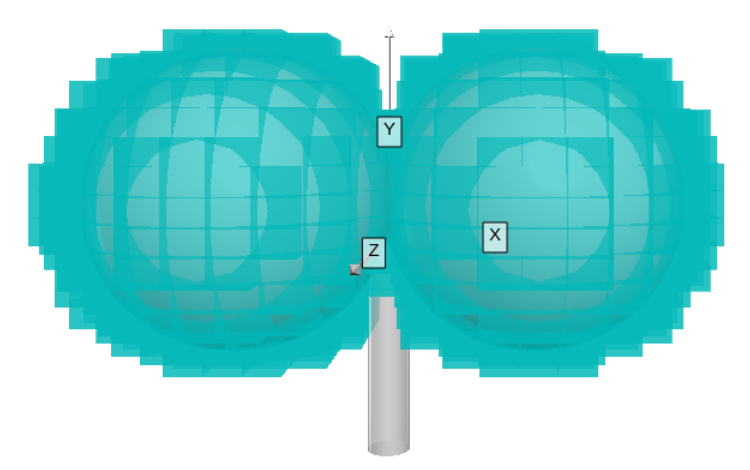
\includegraphics[width = \textwidth]{images/reg_vor}
             \caption{Regular lattice.}
             \label{fig:reg_vor}
        \end{subfigure}
        \hfill
        \begin{subfigure}[b]{0.45\textwidth}
             \centering
             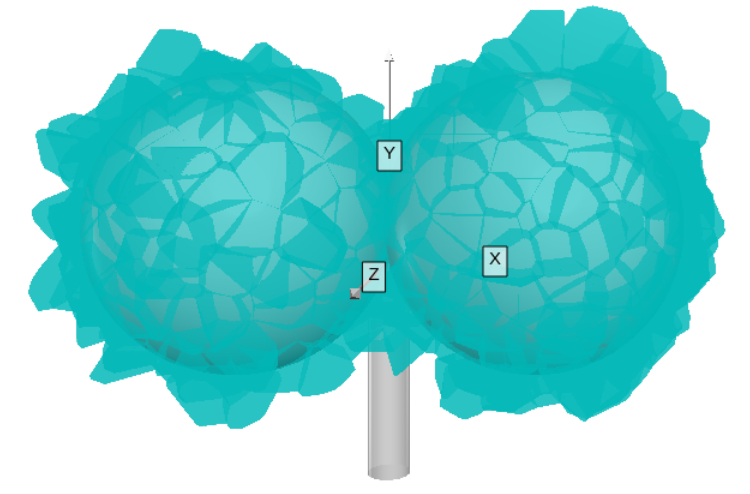
\includegraphics[width = \textwidth]{images/sal_vor}
             \caption{Sampling with Saltelli algorithm.}
             \label{fig:sal_vor}
        \end{subfigure}
        \caption{Comparison between two Voronoi decompositions. The first (left) is created from a regular lattice of starting points, and every piece is exactly equal to all the others, creating a regular subdivision of the space The second (right) is created instead from a sampling made following the Saltelli quasi-random algorithm. The pieces are all different in shape, but they all have similar sizes and volumes. In this pictures in particular have been shown only the pieces of the tessellation which lie in correspondence to the boundaries of the spheres underneath. While watching this picture one should immagine the decomposition extended similarly in all the space around the ramification, within certain boundaries, which loosely contains the structure. This representation choice has been done just for enhance the interpretability of the image. }
        \label{fig:vor_comp}
    \end{figure}

    There are tough some delicate considerations to be highlighted about the decomposition procedure. The first regards the most external pieces of the decomposition. Whilst the internal pieces are neatly bounded and defined, the most external layer instead is made on unbounded regions, which extend themselves to infinity. Those regions have clearly to be rejected, as it would be absurd for a cell to have an infinity volume. Typically those unbounded regions are resized in order to adhere to some limiting boundaries, with an operation known as \textit{cropping}. In Figure \ref{fig:crop_vor} is shown an example of circular cropping in a 2D Voronoi decomposition: all the regions which intersect the circumference have to be resized.

    \begin{figure}
        \centering
        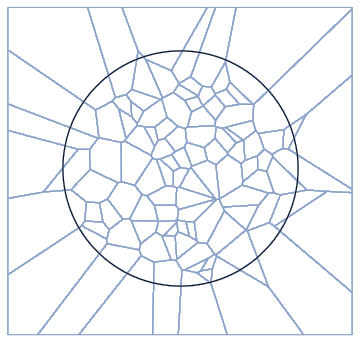
\includegraphics[width = 0.5\textwidth]{images/crop_vor}
        \caption{Example of circular cropping in a 2D Voronoi decomposition: all the regions which intersect the circumference have to be resized.}
        \label{fig:crop_vor}
    \end{figure}

    The cropping operation in 3D is extremely complex, tough. Thus, a more simple and efficient, yet less elegant, technique has been used. Instead of resizing the regions which lie on the boundaries of the sampling region, those regions have directly been rejected. This process is really fast and it does not lead to any danger of representativity loss if the boundaries are loose enough and if the density of sampling is not too low.

    The other important consideration regards the density of sampling points. Increasing the number of points to be extracted from the same volume automatically the number of cells in the box will rise, and in contrast, their relative dimension will decrease. This is a key element of the model: a too rarified decomposition would not bee able to reflect the complexity of the structure underneath, but a too crowd decomposition on the other side would lead to an unrealistic dimension of the cells in the tissue. Furthermore, this parameter has a huge influence on the computing time necessary to generate the model and to process it for the sectioning as will be shown in section \ref{ssec:sectioning}. In almost all the applications so far, the density parameter has been tuned by eye, with a trial and error procedure. Although, a more rigorous way to adjust this parameter would be to consider the average dimension of the cells and make some microanatomical considerations to define the correct relative dimensions. The measure of the volume\footnote{The volume is expressed in the same arbitrary length unit of measures used during the ramification structure. This allows a coherent reference tool.} of the decomposition's regions is an accessible parameter, thus an easy way to estimate the average linear dimension of the cells can be to approximate all the cells to cuboid seeing their volumes as $V \approx L^3$. Averaging all the $L$ measures an estimate $\hat{L}$ can be done. This average length may be compared to the length of the blood vessel ramification, allowing a good reference tool.

    \item [\mycount) Cells Identity Assignment] \hfill \\
    The great power of creating all the models virtually is to know exactly the identity of every point in the structure. Although, This identity has to be reflected at the cellular level, assigning to every region a label. Imagining the Voronoi decomposition represented in Figure  \ref{fig:sal_vor} extended to the entire box containing the ramification, good discrimination would distinguish three classes of cells: those which lie completely inside a sphere, those which lie completely outside a sphere, and those which lie on the boundaries of a sphere. In Figure \ref{fig:cell_id} is shown a portion of the complete decomposition where the three classes of cells are reported with different colors: the internal cells in red, those on the boundaries in turquoise, and the external cells in gray.

    \begin{figure}
        \centering
        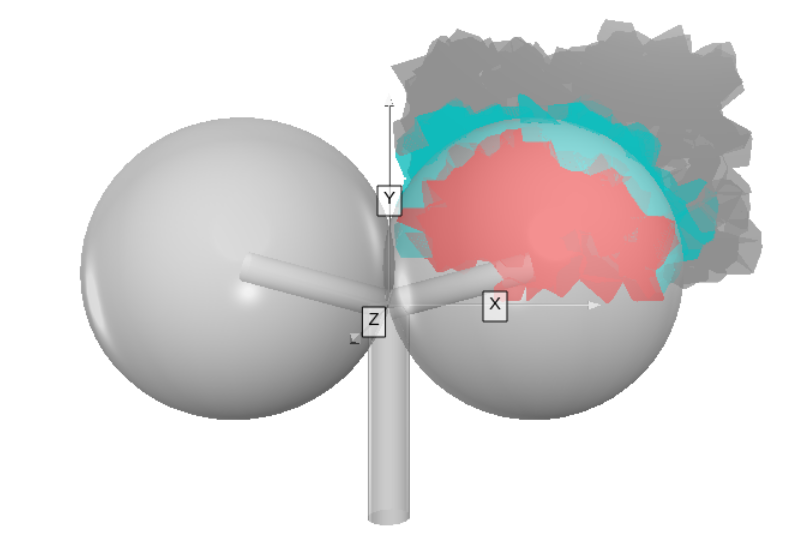
\includegraphics[width = 0.5\textwidth]{images/cell_id}
        \caption{Portion of the complete Voronoi decomposition, showing the three different classes of cell in three different colors: the internal cells in red, those on the boundaries in turquoise and the external cells in gray.}
        \label{fig:cell_id}
    \end{figure}

    In this particular case to find the relative position between every sphere in the structure and each cell it has been used a test on the proximity between the centers and the vertices of every polyhedral cell. If all the vertices of a region lie within a distance lower than the radius from the center of the same sphere then that region can be said to be an internal one. If none of the vertices lie within the radius distance from any center then that region is said to be external. In any other case, the region is said to be on the boundaries of some sphere, and this third label is assigned to it. As could be imagined the number of cells inside the volume can grow very quickly, and in the more rich ramifications also the number of spheres could be high. If we think that any polyhedron has a number of vertices of the order of $20/30$ then it is clear that the number of distance evaluations could grow very quickly, requiring some relevant computational power in the more extended simulations. In order to optimize this computation, I decided to use a python implementation of a K-dimensional Tree, which is a space-partitioning data structure especially suited for fast and optimized computation of distances \cite{10.1145/361002.361007}. A K-d Tree is an algorithm which iteratively binarly splits the space: every node of the three could be thought as a splitting $(k-1)$-hyperplane dividing the space into two semi-hyperspace. The result is an optimized algorithm for repeated distance evaluations. As for many other tools, in my code I used an excellent pre-implemented module \texttt{KDTree} from the \texttt{Scipy} library.

    This procedure of labeling the regions is completely customizable, and it should be adapted to the specific application. By the way, the principle will always be to perform some sort of spatial consideration respect to the primary structure and assign all the interesting labels accordingly to the cells in the volume.
\end{description}

After labeling the cells in the decomposition the model is considered complete. Every enrichment to the structure should be reflected in some type of label for the cells, which are chosen as the fundamental unit in the model. As we will see in section \ref{ssec:sectioning} during the sectioning process in the produced image will be printed mainly the identity of the cells, hence any detail on a finer scale in the model would not be conveyed properly on the final image.

\subsection{Dermal Tissue Model} \label{ssec:panc_tis_mod}
The dermis or corium is a layer of skin between the epidermis (with which it makes up the cutis) and subcutaneous tissues, that primarily consists of dense irregular connective tissue and cushions the body from stress and strain. It is divided into two layers, the superficial area adjacent to the epidermis called the papillary region and a deep thicker area known as the reticular dermis.[1] The dermis is tightly connected to the epidermis through a basement membrane. Structural components of the dermis are collagen, elastic fibers, and extrafibrillar matrix.[2] It also contains mechanoreceptors that provide the sense of touch and thermoreceptors that provide the sense of heat. In addition, hair follicles, sweat glands, sebaceous glands (oil glands), apocrine glands, lymphatic vessels, nerves and blood vessels are present in the dermis. Those blood vessels provide nourishment and waste removal for both dermal and epidermal cells.
    \begin{figure}
        \centering
        \begin{subfigure}[b]{0.45\textwidth}
             \centering
             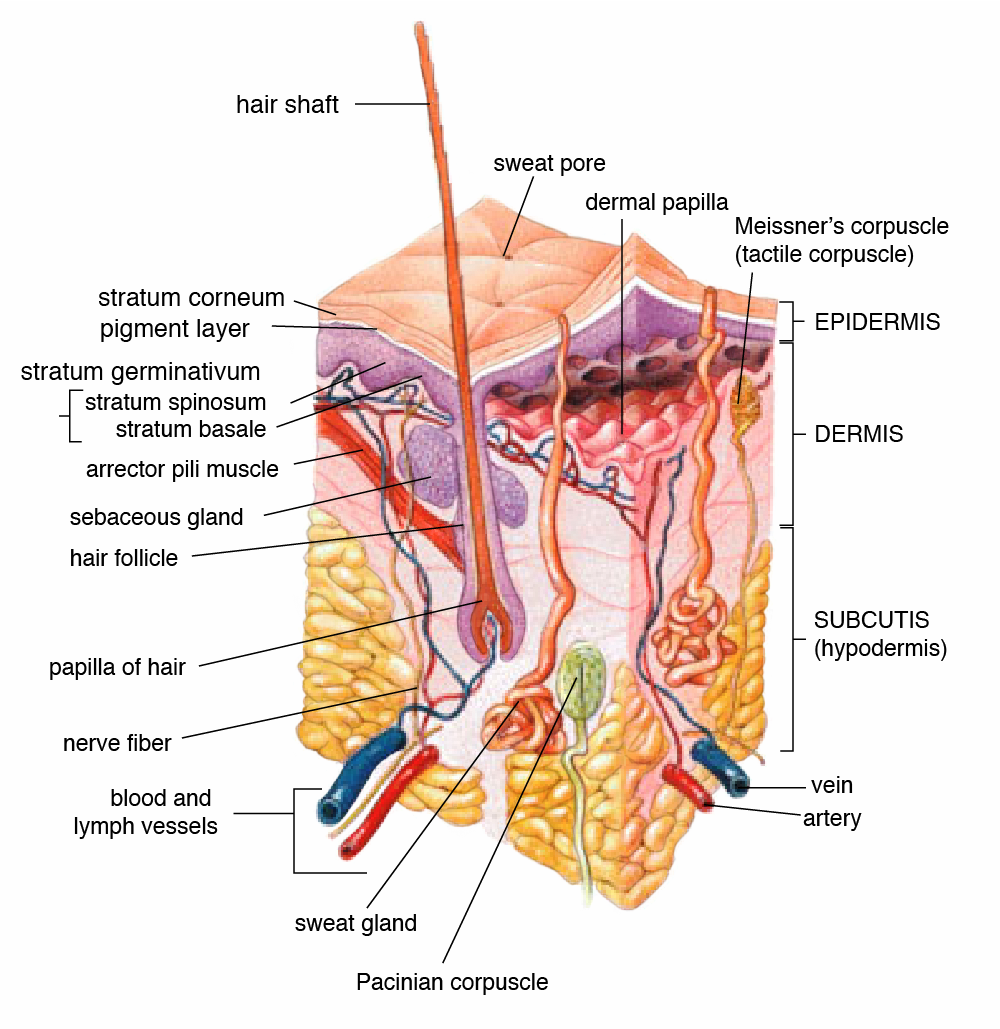
\includegraphics[width = \textwidth]{images/derm_scheme}
             \label{fig:derm_scheme}
        \end{subfigure}
        \hfill
        \begin{subfigure}[b]{0.45\textwidth}
             \centering
             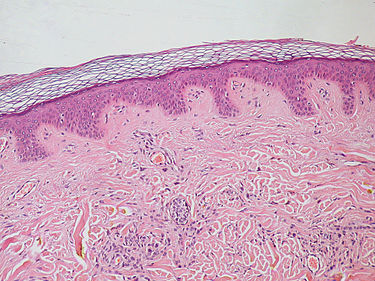
\includegraphics[width = \textwidth]{images/derm_specimen}
             \label{fig:derm_specimen}
        \end{subfigure}
        \caption{Microanatomical description of a region of dermal tissue and all the interesting elements present in cutis, and subcutaneous layer. An actual histological specimen from a sample of dermal tissue.}
        \label{fig:derm_descr}
    \end{figure}


\subsection{Sectioning Process - Synthetic Images} \label{ssec:sectioning}


SECTIONING AND IMAGE PRODUCTION (random direction) -> SEGMENTATION MASK\\
\\
ADJUSTMENTS: PALETTE, NOISE, STYLE TRANSFER\\
\\
PIPELINE TO AUTOMATIZATION\\
ALTERNATIVE METHODS???\\
\clearpage

    \clearpage
    \section{Synthetic Images Production} \label{sec:synth_image}
    After the model is complete we have a three-dimensional representation of the tissue under study. The aim of the work is though to produce synthetic images from that structure, more precisely we want pairs of images composed of the synthetic-histological images and its related segmentation mask. The transition from 3D structure to a 2D image is the last step in the process, and it is inspired by the actual traditional technique for the preparation of the histological specimen, as described back in section \ref{ssec:samp_prep}. As the biopsy sample is treated and then sectioned with the microtome, the virtual model is sectioned in a random direction, producing an image representing the slice. This first image contains all the information of the section but its appearance is completely arbitrary and its look has nothing to share with a realistic sample. The original slice then acts perfectly as a segmentation mask, but some careful and dramatic makeover is needed to produce the final realistic looking image. In this section I will describe the general procedure to produce virtual slices from the two 3D virtual models described before in section \ref{sec:models} and the technique used to edit the images and give them the desired appearance.

\subsection{Sectioning Process} \label{ssec:sect_proc}
    For any model created following the general procedure described in \ref{sec:models}, even more so for the two particular models of pancreatic and dermal tissue, the sectioning process will be almost the same, and it will rely mainly on the algorithm for the general section of polyhedron described back in section \ref{ssec:pol_sec}. As stated before the models are essentially composed by labeled polyhedron spatially organized in a 3D volume. The ordered section of each polyhedron will yield all the polygons that shall be assembled in the final section.
    In Figure \ref{fig:sec_3D} is shown the three-dimensional representation of the section of a simple ramification, as the one in Figure \ref{fig:cell_id}. All the polygons that compose the section are drawn with the color correspondent to their label, following the same idea of Figure \ref{fig:cell_id}. In Figure \ref{fig:section_simple} is printed the final result of the sectioning algorithm applied to the model, which will be the segmentation mask in the single pair of synthetic images. The colors in the produced slice match the colors used for the different identities in the 3D model.

        \begin{figure}[ht]
            \centering
            \begin{subfigure}[t]{0.45\textwidth}
                 \centering
                 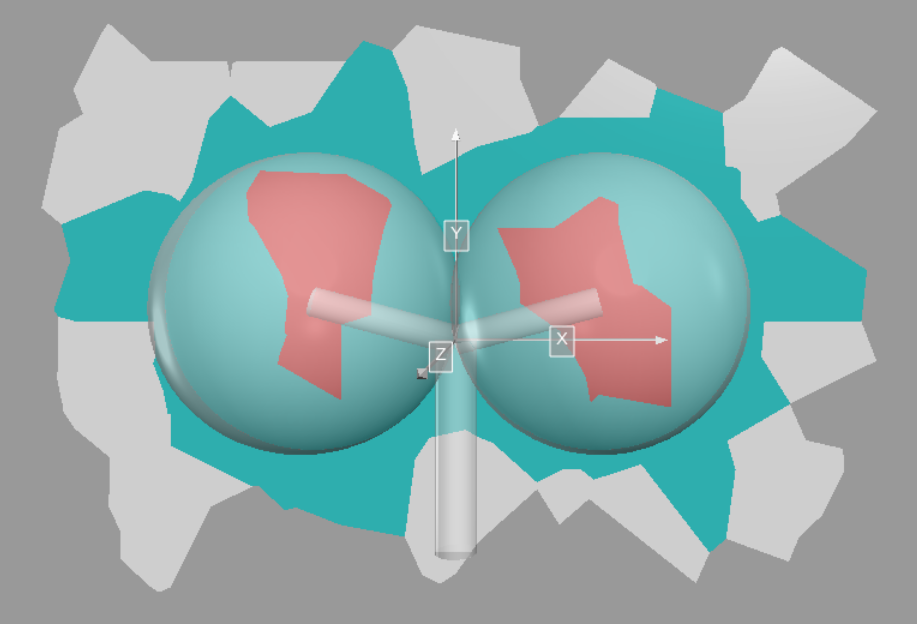
\includegraphics[width = \textwidth]{images/sec_3D}
                 \caption{2D polygonal sections represented in a 3D environment.}
                 \label{fig:sec_3D}
            \end{subfigure}
            \hfill
            \begin{subfigure}[t]{0.45\textwidth}
                 \centering
                 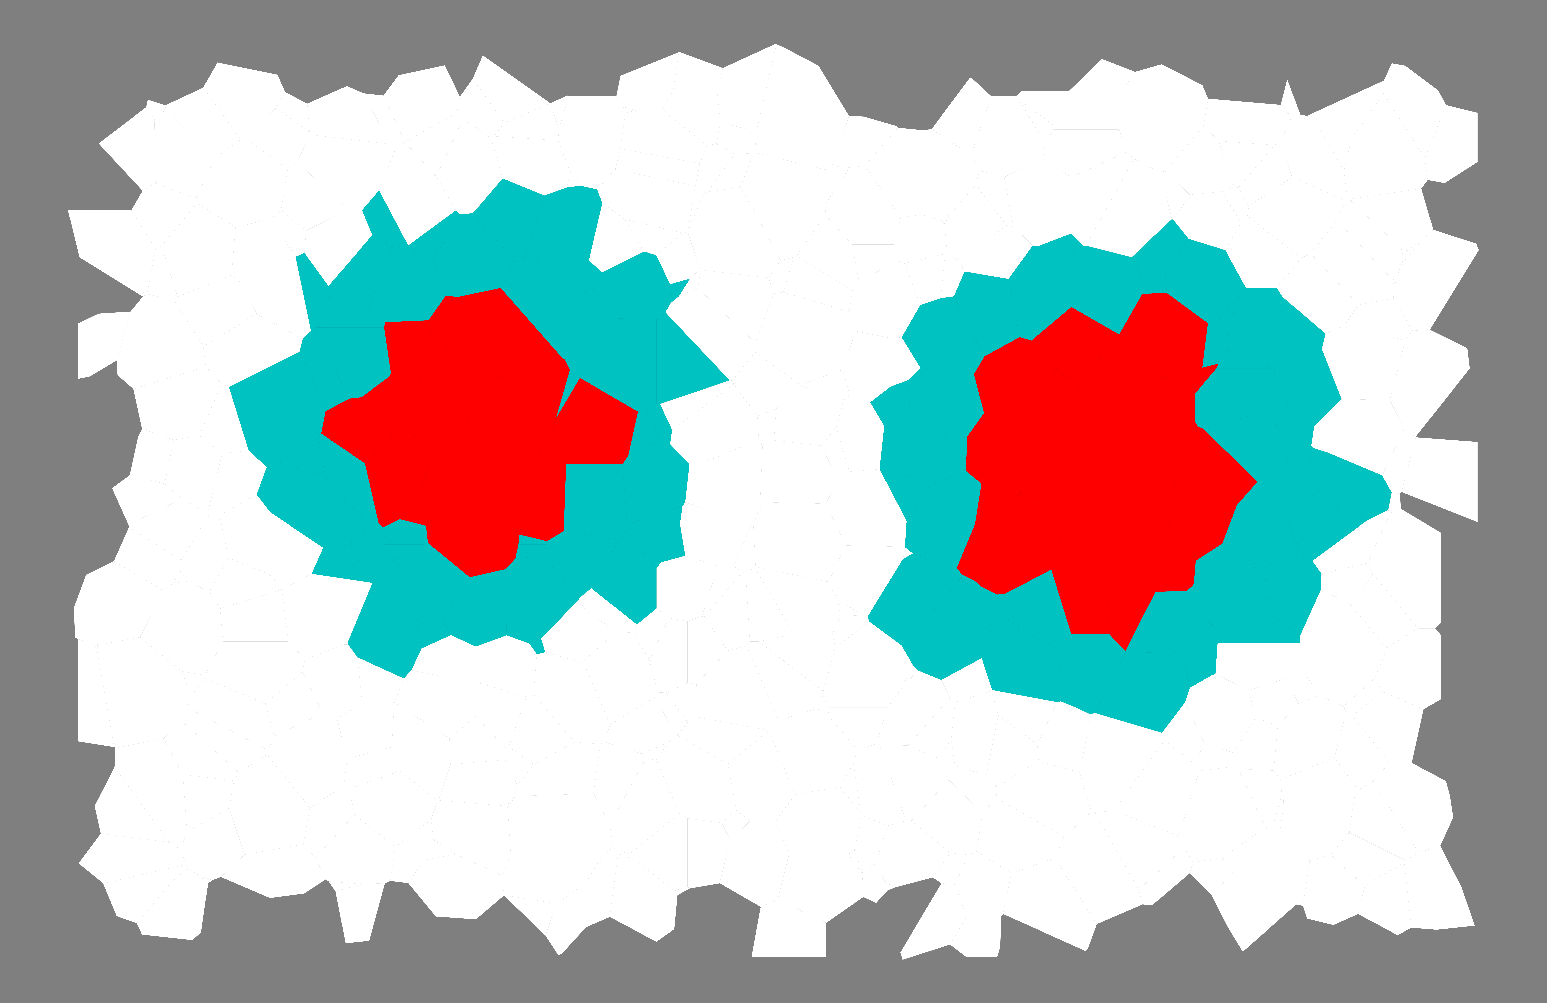
\includegraphics[width = \textwidth]{images/section_simple}
                 \caption{The fianl section image, produced directly on a planar picture, skipping completely the 3D representation.}
                 \label{fig:section_simple}
            \end{subfigure}
            \caption{In this Figure is shown the idea of the correspondence between the section of a simple structure in the space and the correspondent section. The correspondence is not perfect for representation requirments, in fact the two images even if very similar are produced with two completely different methods. At the left an image of 2D polygonal section embeded in a 3D space, made using 3D visualization tools. At the right a simple image produced printing the polygons in a planar picture. Printing 2D polygons in a 3D space is much more complicated than one would think using the same tool used to produce the other images like Figure \ref{fig:cell_id} and \ref{fig:vor_comp}. This choice has been done for the sake of the overall homogeneity in pictures style.}
            \label{fig:first_sect}
        \end{figure}

    The simplest, yet over-abundant, way to proceed is to create the model in its entirety and subsequently choosing the sectioning plane. Afterward, it is necessary to select only the regions that intersect the plane and section them all. Actually, the test on the intersection passes through the check on the relative position of the polyhedron's vertices respect to the sectioning plane: if all the vertices lie on the same semi-space then the intersection would be null and the polyhedron is not of interest for that particular section. This procedure is exactly the first step of the algorithm in \ref{ssec:pol_sec}, thus the filtering on the regions is actually made during construction for optimization. The alternative method could be to choose in the first place the direction of the sectioning plane, and in second place to generate the model's decomposition only in the volume adjacent to that plane. This method enables the sparing of a good amount of computation, without any negative impact on the final result. The only delicate step is the choice of a wide enough region of space around the plane, which doesn't compromise the representation.

    As a guarantee for richness and diversification among the images, there is the need for some degree of controlled randomness in the sectioning process, for example in the determination of the sectioning plane direction. All the sectioning process is then based on a single starting \textit{seed}, which determines the direction of the sectioning plane in a deterministic way, and all the rest of the model is generated as a consequence. In this way, all the possible angulations are equally probable and will be sampled in view of multiple applications of this process. In Figure \ref{fig:4sph_sections} are shown two different sections, along two random planes on two simple ramified structures with four spheres.

        \begin{figure}
            \centering
            \begin{subfigure}[t]{0.2\textwidth}
                 \centering
                 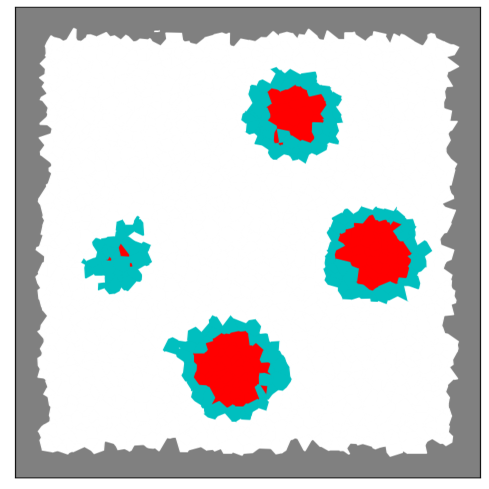
\includegraphics[width = \textwidth]{images/4sph_sec1}
                 \label{fig:4sph_sec1}
            \end{subfigure}
            \quad
            \begin{subfigure}[t]{0.2\textwidth}
                 \centering
                 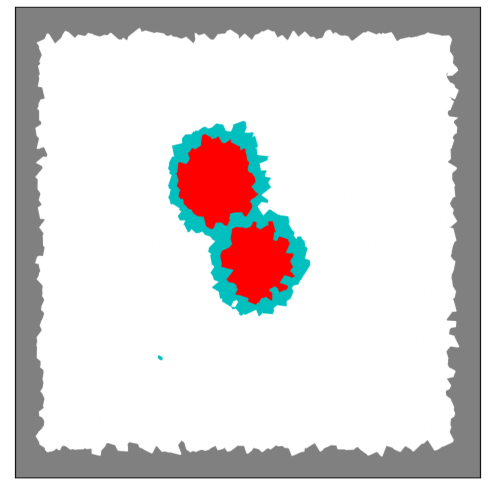
\includegraphics[width = \textwidth]{images/4sph_sec2}
                 \label{fig:4sph_sec2}
            \end{subfigure}
            \caption{Two different section, along two randon planes on two simple ramificated structure with four spheres.}
            \label{fig:4sph_sections}
        \end{figure}

\subsection{Appearance Makeover} \label{ssec:app_mkov}
    After the application of the sectioning algorithm of the previous section, the image which will act as a segmentation mask is ready. The last and most complex task that remains is to transform the image and to give it a realistic look. I tried many different transformations, more or less complicated, and there was not a final decision on which is the best blend of them. In this section, I will describe them as an arsenal of possibilities and show their impact on the images.

    \begin{description}
        \item [Color Palette] \hfill \\
        The first correction to do to the images will inevitably be a change in the colors of the image. Gray, Turquoise, and Red are the perfect choice for label-colors but act poorly as physiological colors. In Figure \ref{fig:new_palette} is shown an example of an image produced re-mapping the colors to a new palette, inspired to the coloring of the real specimen in Figure \ref{fig:panc_struct} and \ref{fig:he_retyna}, given by the traditional hematoxylin and eosin staining process.

        \begin{figure}[h]
            \centering
            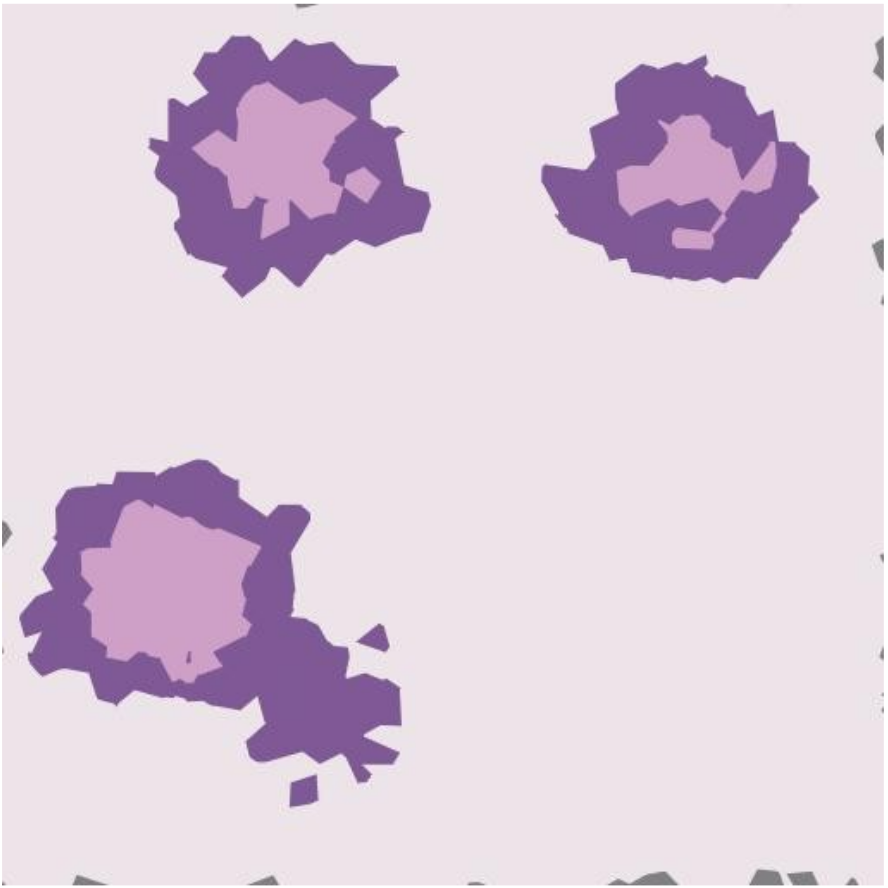
\includegraphics[width = 0.2\textwidth]{images/new_palette}
            \caption{Example of images produced re-mapping the colors with a color palette inspired to a real H\&E stained histological sample.}
            \label{fig:new_palette}
        \end{figure}

        \item [Nuclei Projection] \hfill \\
        Another fundamental processing needed was the projection of cells' nuclei on the image. Usually, nuclei are clearly visible in histological samples and guide the analysis allowing to detect individual cells in the specimen. As a reference for the nucleus position the starting point of every polyhedral region has been used and projected on the sectioning plane as a little dark circle. The diameter of those circles as been chosen to be a submultiple (10\%) of the linear estimated dimension $\hat{L}$ of the cells in the decomposition\footnote{Following the same logic of step 3 of section \ref{ssec:panc_tis_mod}.}.

        \begin{figure}
            \centering
            \begin{subfigure}[t]{0.2\textwidth}
                 \centering
                 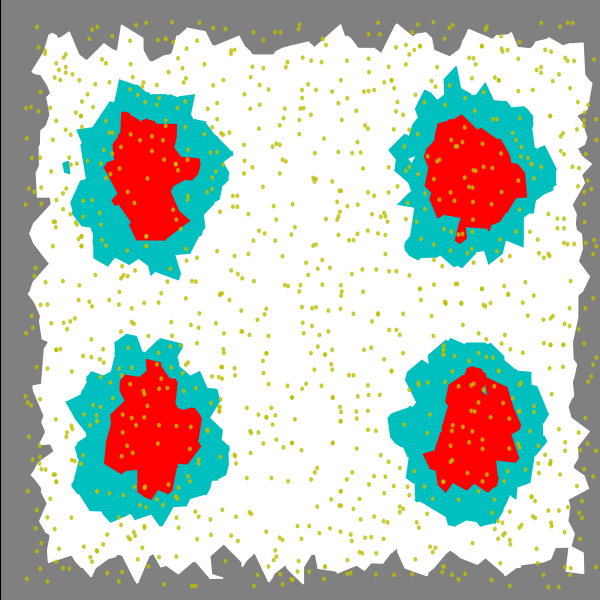
\includegraphics[width = \textwidth]{images/nuclei_mask}
                 \label{fig:nuclei_mask}
            \end{subfigure}
            \quad
            \begin{subfigure}[t]{0.2\textwidth}
                 \centering
                 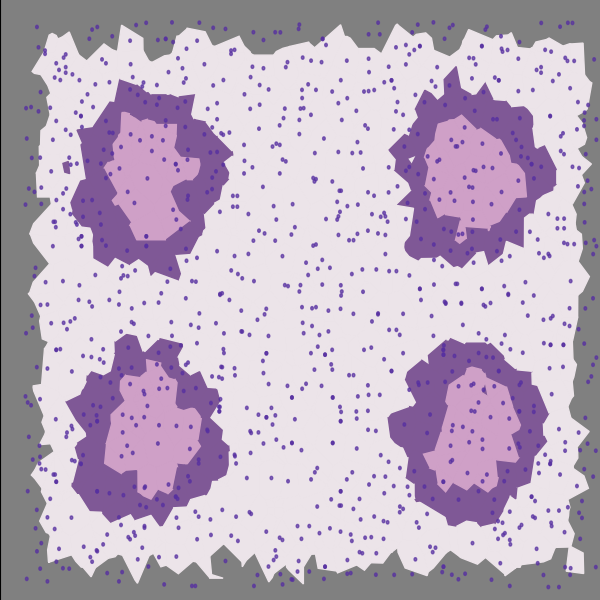
\includegraphics[width = \textwidth]{images/nuclei_real}
                 \label{fig:nuclei_real}
            \end{subfigure}
            \caption{Nuclei projection on the image: (left) in yellow in the segmentation mask and (right) in purple in the image under makeover.}
            \label{fig:nuclei_proj}
        \end{figure}

        Nuclei projection, among the other things, is an excellent tool to perceive the different effects obtained with different choices of quasi-random distributions or fully-random distributions (with reference to section \ref{ssec:saltelli}). The different impact on the overall image is huge, and it really changes the overall sense of the image. In Figure \ref{fig:sampling_comparison} are reported four different sections, produced with the same density on cells but with four different methods for the sampling of starting decomposition's points.

        \begin{figure}
            \centering
            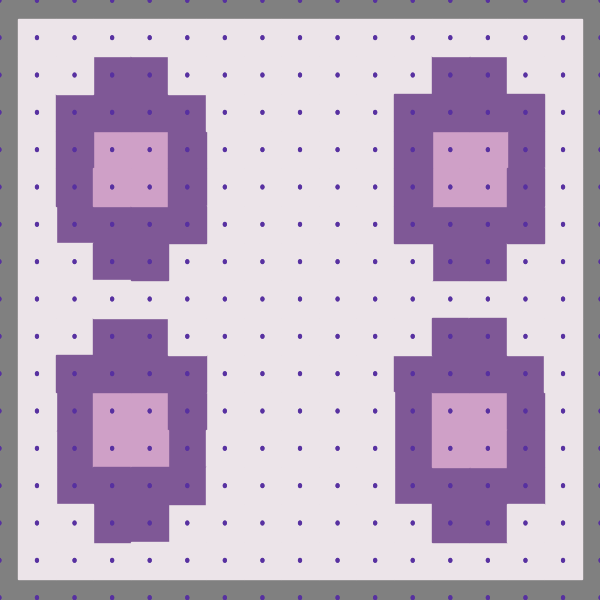
\includegraphics[width =0.24 \textwidth]{images/lattice}
            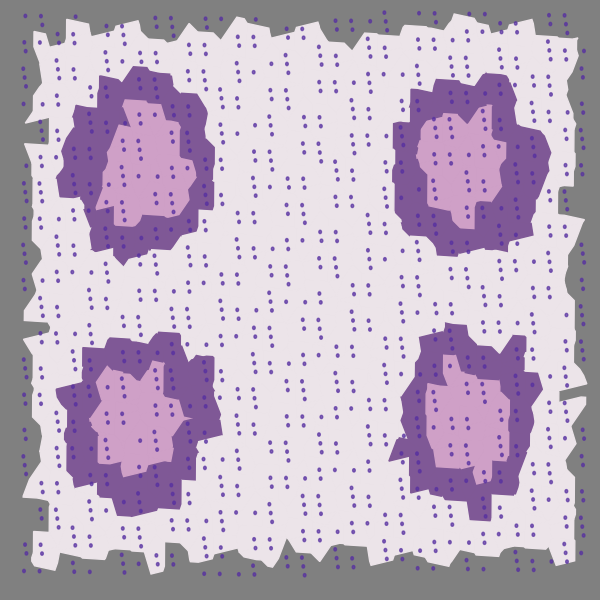
\includegraphics[width =0.24 \textwidth]{images/sequence}
            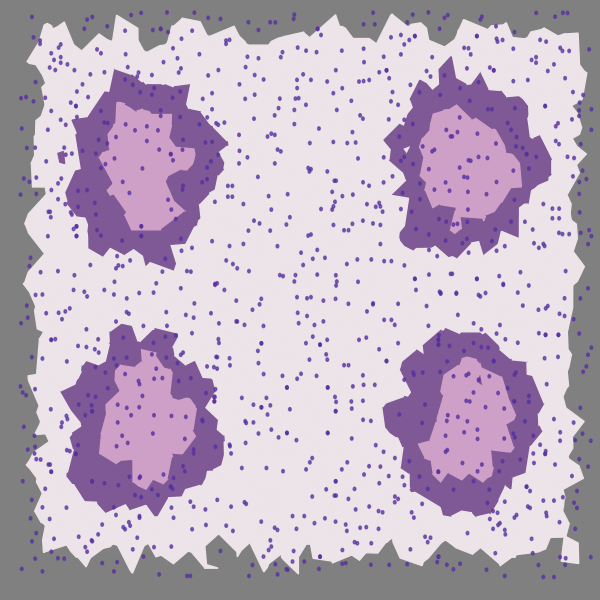
\includegraphics[width =0.24 \textwidth]{images/saltelli}
            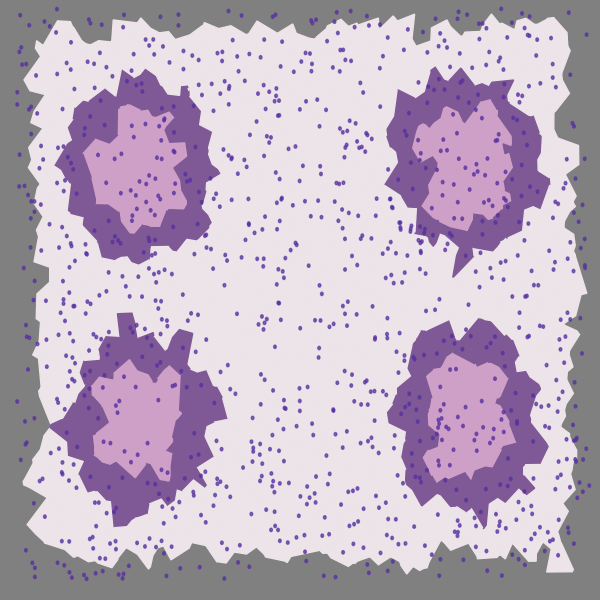
\includegraphics[width =0.24 \textwidth]{images/uniform}
            \caption{Four different sections produced with the same density on cells but with four different method for the sampling of starting decomposition's ponits (from left to right): $\bullet$ points sampled on a regular lattice, $\bullet$ sampling following a simple recursion sequence as the one in equation (\ref{eq:ad_rec}), $\bullet$ following the \textit{saltelli} algorithm, $\bullet$ following a fully-random distribution.}
            \label{fig:sampling_comparison}
        \end{figure}

        \item [Boundaries Projection] \hfill \\
        On the same wave of the previous tool, another operation that can help the appearance of an image is the projection of the boundaries of each (or just a part) of the polygonal sections. The drawing can be clearly tuned and customized depending on the specific necessities. In Figure \ref{fig:derma_slice} is shown an example of a section on the dermal tissue model in \ref{ssec:derm_tis_mod}, in which the boundaries of all the cells have been lightly marked, and the boundaries of the cells in the keratine layer have been heavily marked instead.

        \begin{figure}
            \centering
            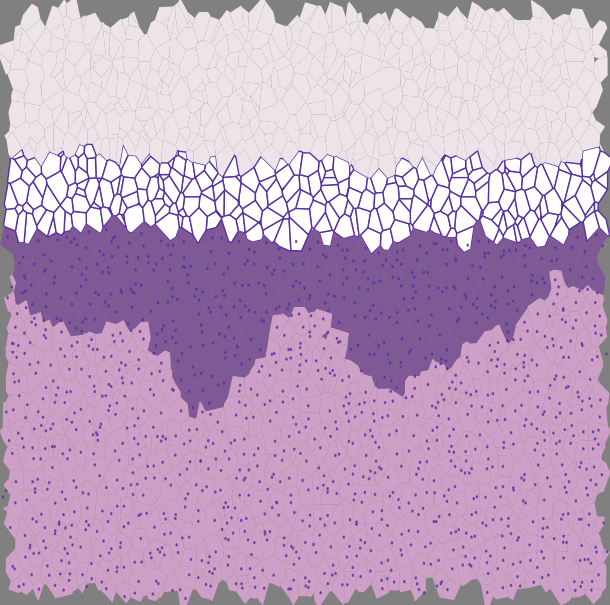
\includegraphics[width = 0.4\textwidth]{images/derma_slice}
            \caption{Example of images produced re-mapping the colors with a color palette inspired to a real H\&E stained histological sample.}
            \label{fig:derma_slice}
        \end{figure}

        \item [Blurring Effects] \hfill \\
        In all the images produced so far the boundaries between polygonal sections are perfectly sharp and without any smudge. To give a more realistic feeling to those pictures I tried different forms of blurring. As a first try, I applied a Gaussian blurring filter, which is an extremely common blurring operation in computer vision, which consists of a simple discrete convolution with a 2D Gaussian kernel. The effect is a regular and diffuse blur all over the image, as in Figure \ref{fig:gauss_blurr}. The second blurring effect I implemented was based instead on the averaging of parallel and adjacent slices on the same model. This method is inspired by the real sectioning technique (section \ref{ssec:samp_prep}), in which every slice is not an infinitesimal layer of matter, but a finite sample, which suffers from mechanical dragging during the process. The idea is that the average between three or more slices equally spaced above and below the \textit{main} slice should recreate a realistic blurring effect. An example of an image produced with this process is shown in Figure \ref{fig:av_blur}.

        \begin{figure}
            \centering
            \begin{subfigure}[t]{0.3\textwidth}
                 \centering
                 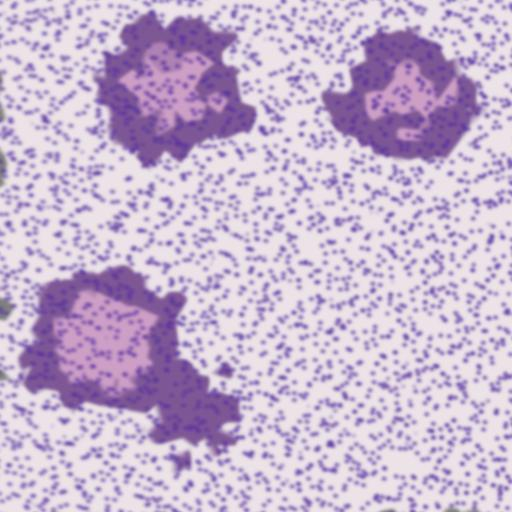
\includegraphics[width = \textwidth]{images/gauss_blurr}
                 \caption{}
                 \label{fig:gauss_blurr}
            \end{subfigure}
            \quad
            \begin{subfigure}[t]{0.3\textwidth}
                 \centering
                 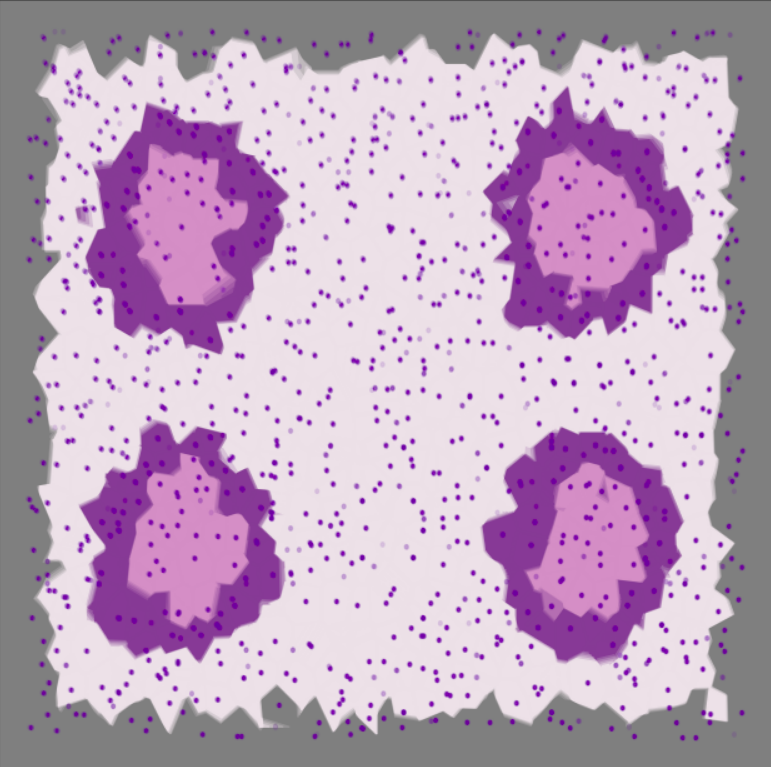
\includegraphics[width = \textwidth]{images/average}
                 \caption{}
                 \label{fig:av_blur}
            \end{subfigure}
            \quad
            \begin{subfigure}[t]{0.3\textwidth}
                 \centering
                 
\includegraphics[width = \textwidth]{images/rgb_prlin}
                 \caption{}
                 \label{fig:rgb_prlin}
            \end{subfigure}

            \caption{The two blurring effects used in this work: (left) A standard Gaussian-filter blur and (center) a specific blur introduced averaging adjacent parallel slices on the same image, (right) an example of RGB color noise built joining three different Perlin noise surfaces, one for each color channel.}
            \label{fig:blur_effect}
        \end{figure}

        \item [Perlin RGB Noise] \hfill \\
        A further attempt to give visual texture to the image was done using again the Perlin noise, described in section \ref{ssec:perlin}. The idea is to create some fluctuation among the color channels of the image around the sharp values of the image produced by the sectioning algorithm.
        From a practical point of view, I created three different and independent Perlin noise surfaces, one for every color channel (Red, Green, and Blue), and added them to create an RGB noise on the image. An example of the resulting image is shown in Figure \ref{fig:rgb_prlin}.

        \item [Style Transfer] \hfill \\
        This last tool I will describe is the most sophisticated so far. It consists of the application of a style-transfer neural network (STNN) on the image obtained through the sectioning process, for the implantation of the visual texture from a real sample of the corresponding tissue. Style-transfer NNs, and their functioning, have been described in detail in section \ref{ssec:sttrNN}, and here I will cover just the particular applications on the two type of section produced.

        The first manipulation I report is the one on a section from the pancreatic tissue model. The image of which to conserve the visual content is a section with some simple pre-processing picked from the ones described before (Figure \ref{fig:st_nn1}): a more accurate color palette, the projection of nuclei, and the average on five adjacent slices. The image from which to pick the style, thus the visual texture, is a portion of an actual histological sample of the pancreas, and it is shown in Figure \ref{fig:st_nn2}. The application of the STNN yields a hybrid image, shown in Figure \ref{fig:st_nn3}. The second application was made on a section on dermal tissue. The three content, style and styled images are shown respectively in Figure \ref{fig:st_nn4}, \ref{fig:st_nn5}, and \ref{fig:st_nn6}.

        \begin{figure}
            \centering
            \begin{subfigure}[t]{0.3\textwidth}
                 \centering
                 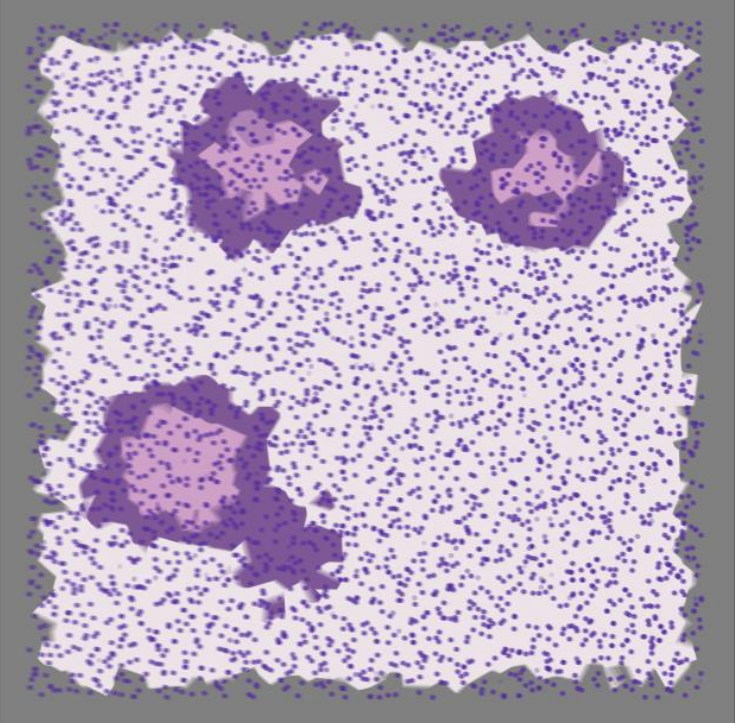
\includegraphics[width = \textwidth]{images/st_nn1}
                 \caption{}
                 \label{fig:st_nn1}
            \end{subfigure}
            \quad
            \begin{subfigure}[t]{0.3\textwidth}
                 \centering
                 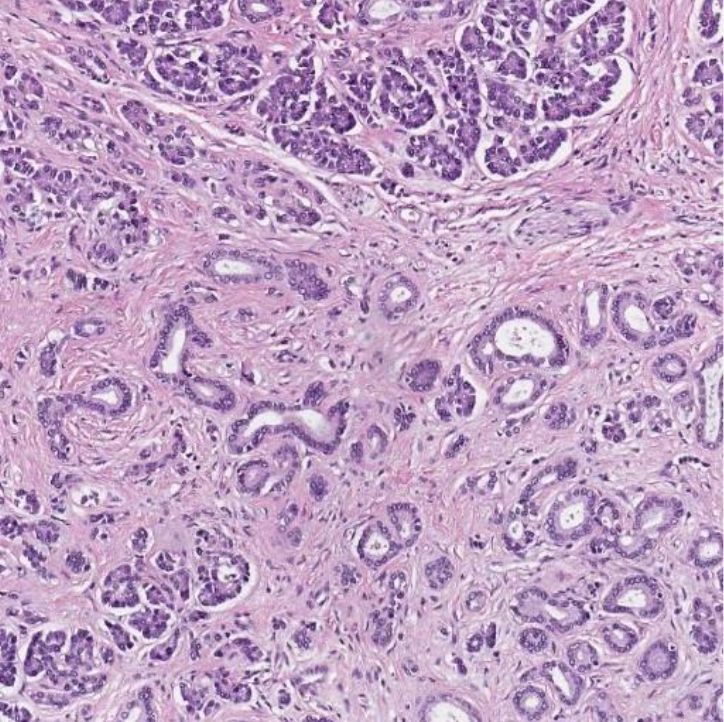
\includegraphics[width = \textwidth]{images/st_nn2}
                 \caption{}
                 \label{fig:st_nn2}
            \end{subfigure}
            \quad
            \begin{subfigure}[t]{0.3\textwidth}
                 \centering
                 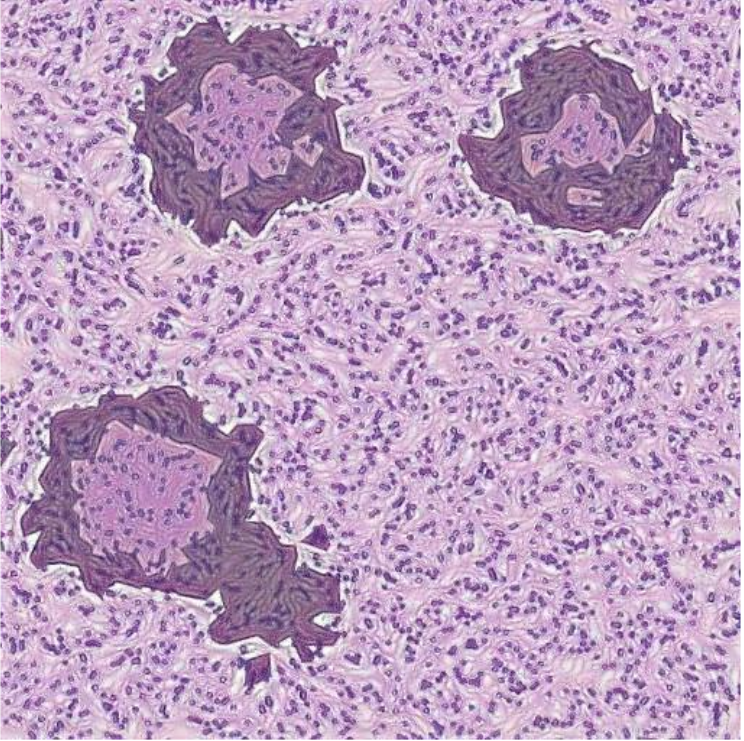
\includegraphics[width = \textwidth]{images/st_nn3}
                 \caption{}
                 \label{fig:st_nn3}
            \end{subfigure}
            \caption{Application of the style-transfer NN on a section of the pancreatic tissue model: \ref{fig:st_nn1} the content image, \ref{fig:st_nn2} the style image, \ref{fig:st_nn3} the hybrid resulting image.}
            \label{fig:panc_stnn}
        \end{figure}

        In Figures \ref{fig:panc_stnn}, and \ref{fig:derm_stnn} are reported the best results among all the different tests made on the sections. I made different tries on the same image with different processing before the manipulation with the STNN, to see the impact of the different adjustment on the resulting styled image. It turned out that the presence of nuclei is essential to give a homogeneous texture to the image and avoid unrealistic artifacts. On the other hand, the choice of the color palette has a way lighter effet than what one would think: the model yields almost the same result with a grey-levels image or with any other palette.

        It interesting to notice the timing cost of this style transfer operation. While all the other manipulation described in this chapter requires a very short time (seconds) to be applied, and are in practice \textit{instantaneous}, the transfer of style is a way more robust operation, which implies the finalization of the training of a pre-trained neural network. On a computer with the technical specification described in section \ref{ssec:my_machine} this operation instead took minutes, which is a time two full orders of magnitude greater.

        \begin{figure}
            \centering
            \begin{subfigure}[t]{0.3\textwidth}
                 \centering
                 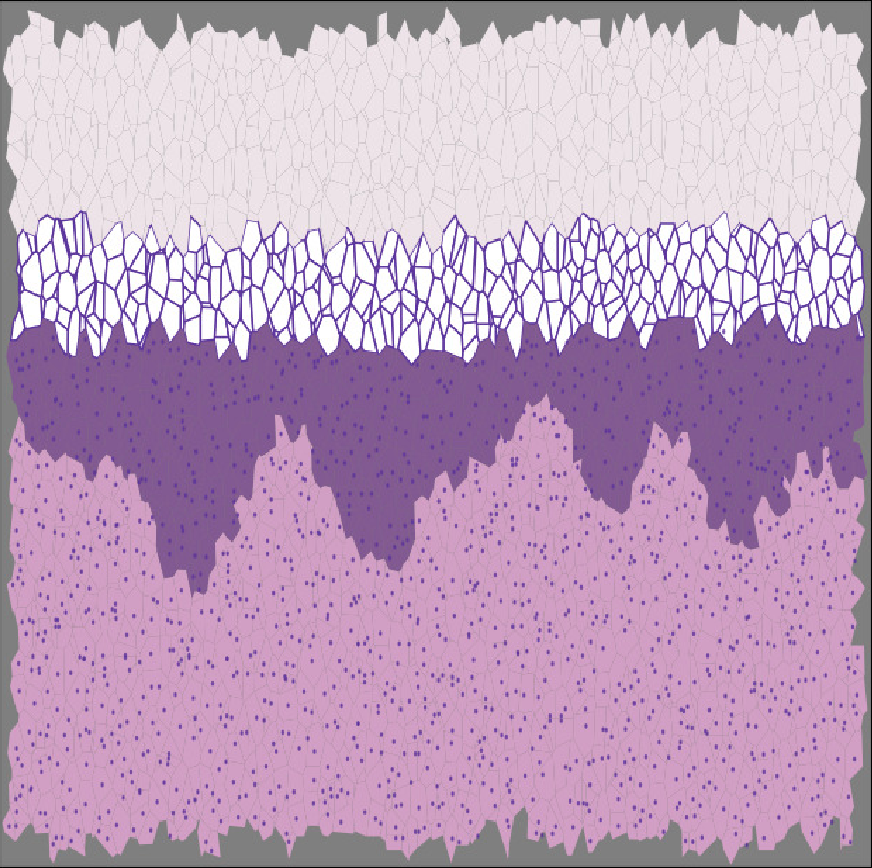
\includegraphics[width = \textwidth]{images/st_nn4}
                 \caption{}
                 \label{fig:st_nn4}
            \end{subfigure}
            \quad
            \begin{subfigure}[t]{0.3\textwidth}
                 \centering
                 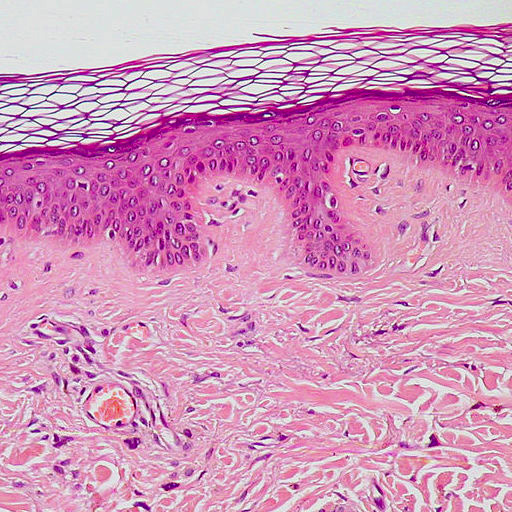
\includegraphics[width = \textwidth]{images/st_nn5}
                 \caption{}
                 \label{fig:st_nn5}
            \end{subfigure}
            \quad
            \begin{subfigure}[t]{0.3\textwidth}
                 \centering
                 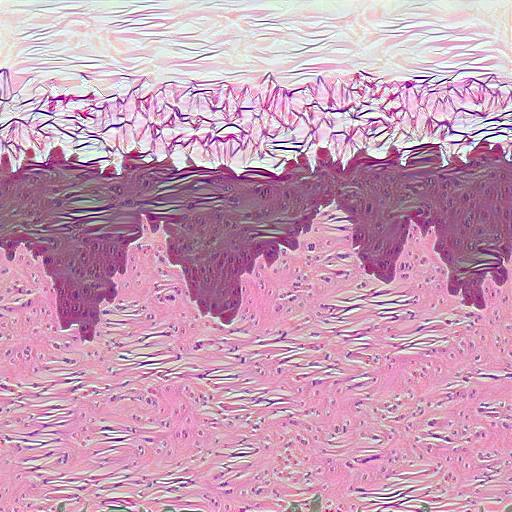
\includegraphics[width = \textwidth]{images/st_nn6}
                 \caption{}
                 \label{fig:st_nn6}
            \end{subfigure}
            \caption{Application of the style-transfer NN on a section of the dermal tissue model: \ref{fig:st_nn4} the content image, \ref{fig:st_nn5} the style image, \ref{fig:st_nn6} the hybrid resulting image.}
            \label{fig:derm_stnn}
        \end{figure}

        It should be noted that the presented results are obtained from the application of a pre-trained STNN model. The development of a specialized model for histological texture transfer could improve extremely the ability to produce realistic images, way further the present results.
    \end{description}

One single complete application of the process consists then in the generation of a tissue model, in the sectioning along a random section plane, and in the processing of the image, in order to produce the pair of ground-truth image and the synthetic histological image. The target is to apply over and over this process to collect the necessary amount of images and constitute an entire dataset. An important feature to have for the process is thus a complete automatization, in order to scale up the generation of images, possibly even in parallel computation.
For this purpose, I created a pipeline workflow interface for the image generation, with an automatized harmonization of every piece of the process. The generation now requires just to fill a configuration file in which writes all the specific characteristics of the images: the type of structure, its features, the desired processing on the images, and eventually the random seeds for a supervised generation. In Figure \ref{fig:dataset} is reported a small scale example of a dataset produced with multiple automatized applications of the generation tool on a ramified structure inspired to a pancreatic tissue model. It is clear the correspondence between segmentation mask and synthetic histological images, and the diversification given by the supervised randomness on the generation.

The actual tool used for the set up of a working pipeline was the \texttt{Snakemake} \cite{10.1093/bioinformatics/bts480} workflow management system, which is a python-based tool to create reproducible and scalable data analyses.

    \begin{figure}
        \centering
        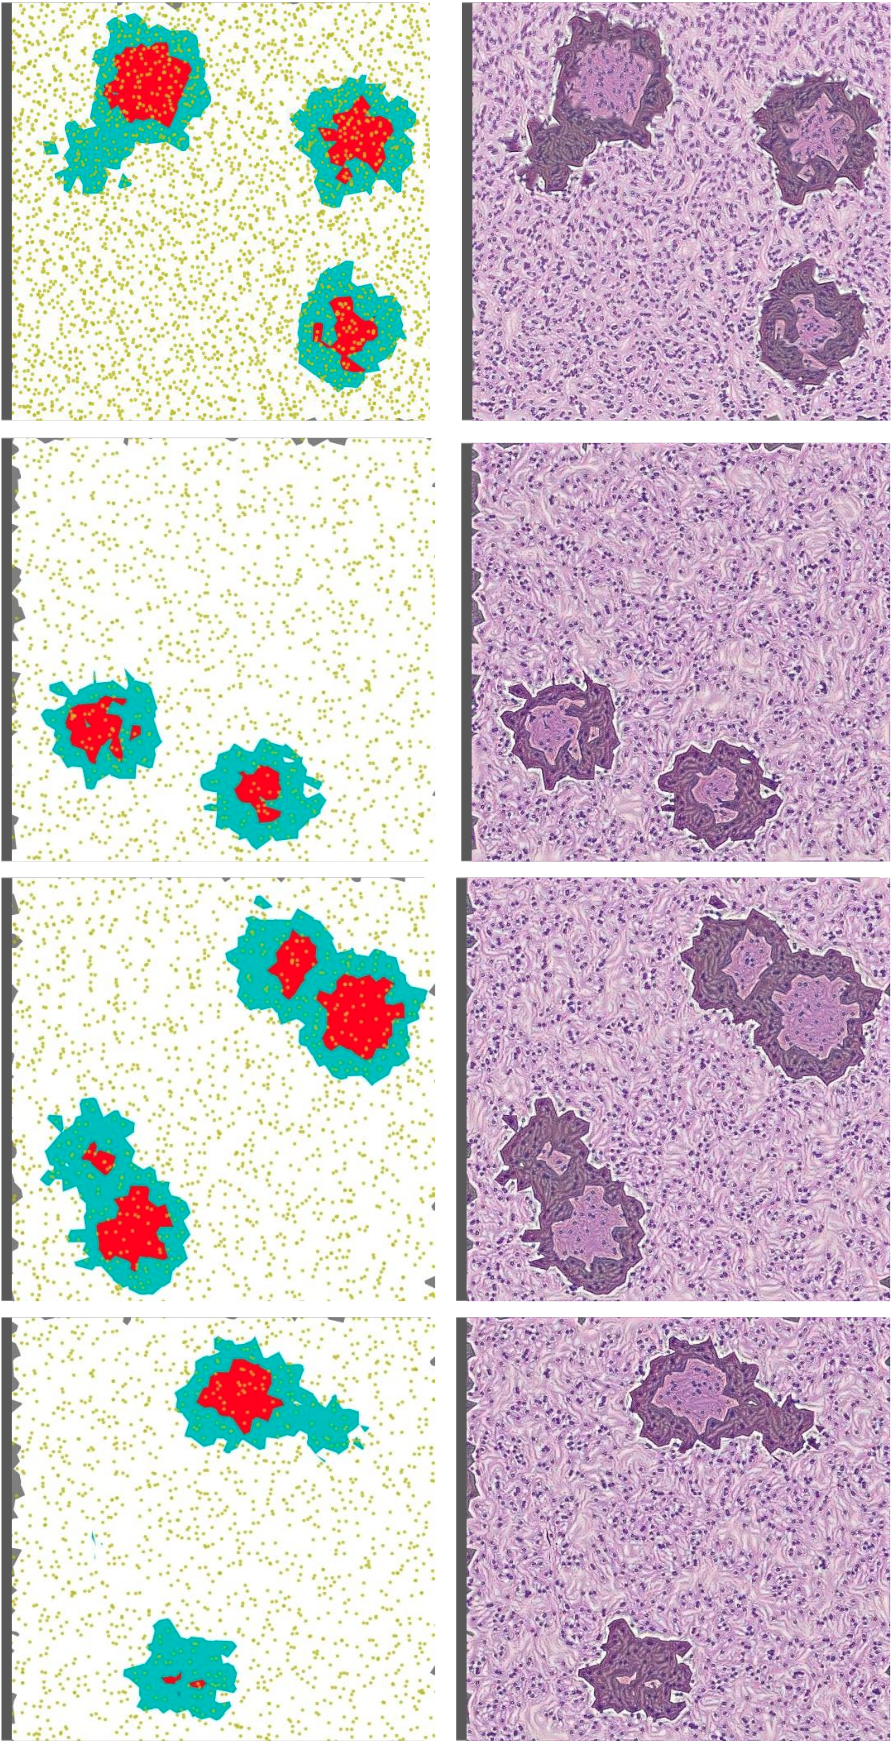
\includegraphics[height=20cm,keepaspectratio]{images/dataset}
        \caption{Small scale example of dataset produced with multiple automatized applications of the generation tool on a ramificated structure inspired to a pancreatic tissue model.}
        \label{fig:dataset}
    \end{figure}

    \clearpage

\chapter*{Conclusions}
\label{chap:concl}
\addcontentsline{toc}{chapter}{\nameref{chap:concl}} %manually adding the unnumbered chapter to toc

In this project I face the problematic of synthetic histological image generation for the purpose of training Neural Networks for the segmentation of real histological images. The manual analysis of histological specimen is a complex, time consuming, and expensive task even if it is a pillar of countless diagnostic techniques. Any form of support for this procedure hence is welcome and endorsed by the health-care system. In particular in this work I focus on the problem of specimens segmentation and its automatization. The most advanced algorithms for image segmentation are based on Deep Learning, and requires the training of extensive and complex neural networks. One of the toughest hurdle to overcome for the training of those NN is the abboundacy and the quantity of pre-labeled example of segmentation on real histological samples. The collection of hundreds of hand-labeled histological samples, with a pixel-level precision is virtually impossible. This work thus proposes a metodology to generate, in a complete automatic way, synthetic pre-labeled histological-like images, that can be used as training material for those NN.

The method I propose consists of the recreation of the traditional histological specimes' preparation, thus is based on the sectioning of a 3D virtual model of a region of histological tissue. The 3D model of a region of a particular type of human tissue is based on physical and physiological considerations, and virtualized. The model is then subject to a virtual sectioning operation, which yields the synthetic sampling of the virtual tissue in which the histological identity of every pixel is perfectly know. This first image will act as segmentation mask for the second, realistic image. In fact, on top of this first image are applied several aesthetical processing and refinments and the final product is the synthetic histological-like image. The pair made of the two images is then perfect for the supervised learning of a NN oriented toward the segmentation of histological images. The production of each pair of images is completely automatic and it does not require the intervention of any human operator, it is thus a scalable process which can produce a great abundance of images. The quality of the images is directly connected to the richness and the quality of the model. The perfect modelization of a region of tissue, let's say human pancreatic tissue, is by far out of reach for this, hence the richness and the fidelity of the produced images is inevitably lower than the real sample. Nevertheless, the quality of the produced images is sufficient to perform the preliminary phase of the training of a NN following a training strategy known as curriculum learning. This learning process consists of giving the NN a copious quantity of lower complexity level example in first instance, reserving the few and sophisticated real hand-labeled histological samples for the finalization of the training.

The first chapter of this thesis is devoted to the contestualization of the present work. It is offered a description of how the histological samples are obtained after a tissue biopsy and how the digitalization process of the images works. The reader is then introduced to the framework of Deep Learing, its fundamental aspect and components. The concept of NN is exposed and it is given the general idea hunderneath the training of a DL-based model. The chapter comes to an end with a general introduction to the segmentation task in computer vision, and how it is currently tackled with state-of-the-art algorithms.

The second chapter collects all the details of every less common technical tool I used during the design of this project. A brief theoretical introduction is proposed for every item besides the thouroug descriprion of its practical use. Some of the arguments touched by this chapter are: quaternions, quasi-random number generation, Voronoi decomposition, style transfer neural networks. In this chapter a section is devoted to the description of a general methodology for computing the 2D section of an arbitray three-dimensional polyhedron. The algorithm here described has been devised and implemented by my self, and then inserted in the workflow of the project. As a conclusion for this chapter I describe the working environment I built for developing this project and the mention of all the code libraries I employeed in my work.

The third chapter is the heart of this work, and it contains the description of all the design choices, and the steps I followed for the development of the two human tissue models I propose: the first of pancreatic tissue and the second of dermal tissue. The development has required the harmonization of many different technical aspects and mathematical tools. The first section is then dedicated to the description of the pancreatic tissue model, which passes through different steps: from a two-dimensional ramification taken as inspiration for the behaviur of blood vessels to the complete three-dimensional model, with its subdivision in labeled cells. The second section is occupied by the description of the dermal tissue model, following the same spirit. The third section instead contains the thorough description of the method to perform the sectioning onto a virtual model and how to process the resulting images. It is necessary to perfom several alternative processing and adjustment to achieve the desired aspect both for the segmentation mask image and for the histologicl-like image.

\hl{The method I propose here for the generation of datasets of synthetic images is self-supporting and ready to work}. By the way, there are many possibilities of improvment and enrichment for the project. One first aspect to strengthen could be the richenss of the models and the collection of available models: adding more elements in the structure and imporving the representation of the cellular level functioning. This would lead to a better quality and representativeness of the synthetic images, that would assist the training of NN in more and different applications. Another aspect that lends itself to improvments is the deveopment of a dedicated style transfer NN targeting the histological texture transfer, which could lead to interesting progresses in the quality of image generation.

There is also the intention to perform an actual attempt of NN training on the images produced with this process. This would be 

\clearpage

\bibliography{biblio}
\end{document}
